\documentclass[twoside]{book}

% Packages required by doxygen
\usepackage{calc}
\usepackage{doxygen}
\usepackage{graphicx}
\usepackage[utf8]{inputenc}
\usepackage{makeidx}
\usepackage{multicol}
\usepackage{multirow}
\usepackage{textcomp}
\usepackage[table]{xcolor}

% Font selection
\usepackage[T1]{fontenc}
\usepackage{mathptmx}
\usepackage[scaled=.90]{helvet}
\usepackage{courier}
\usepackage{amssymb}
\usepackage{sectsty}
\renewcommand{\familydefault}{\sfdefault}
\allsectionsfont{%
  \fontseries{bc}\selectfont%
  \color{darkgray}%
}
\renewcommand{\DoxyLabelFont}{%
  \fontseries{bc}\selectfont%
  \color{darkgray}%
}

% Page & text layout
\usepackage{geometry}
\geometry{%
  a4paper,%
  top=2.5cm,%
  bottom=2.5cm,%
  left=2.5cm,%
  right=2.5cm%
}
\tolerance=750
\hfuzz=15pt
\hbadness=750
\setlength{\emergencystretch}{15pt}
\setlength{\parindent}{0cm}
\setlength{\parskip}{0.2cm}
\makeatletter
\renewcommand{\paragraph}{%
  \@startsection{paragraph}{4}{0ex}{-1.0ex}{1.0ex}{%
    \normalfont\normalsize\bfseries\SS@parafont%
  }%
}
\renewcommand{\subparagraph}{%
  \@startsection{subparagraph}{5}{0ex}{-1.0ex}{1.0ex}{%
    \normalfont\normalsize\bfseries\SS@subparafont%
  }%
}
\makeatother

% Headers & footers
\usepackage{fancyhdr}
\pagestyle{fancyplain}
\fancyhead[LE]{\fancyplain{}{\bfseries\thepage}}
\fancyhead[CE]{\fancyplain{}{}}
\fancyhead[RE]{\fancyplain{}{\bfseries\leftmark}}
\fancyhead[LO]{\fancyplain{}{\bfseries\rightmark}}
\fancyhead[CO]{\fancyplain{}{}}
\fancyhead[RO]{\fancyplain{}{\bfseries\thepage}}
\fancyfoot[LE]{\fancyplain{}{}}
\fancyfoot[CE]{\fancyplain{}{}}
\fancyfoot[RE]{\fancyplain{}{\bfseries\scriptsize Generated on Mon Oct 28 2013 17\-:33\-:55 for Pacman by Doxygen }}
\fancyfoot[LO]{\fancyplain{}{\bfseries\scriptsize Generated on Mon Oct 28 2013 17\-:33\-:55 for Pacman by Doxygen }}
\fancyfoot[CO]{\fancyplain{}{}}
\fancyfoot[RO]{\fancyplain{}{}}
\renewcommand{\footrulewidth}{0.4pt}
\renewcommand{\chaptermark}[1]{%
  \markboth{#1}{}%
}
\renewcommand{\sectionmark}[1]{%
  \markright{\thesection\ #1}%
}

% Indices & bibliography
\usepackage{natbib}
\usepackage[titles]{tocloft}
\setcounter{tocdepth}{3}
\setcounter{secnumdepth}{5}
\makeindex

% Hyperlinks (required, but should be loaded last)
\usepackage{ifpdf}
\ifpdf
  \usepackage[pdftex,pagebackref=true]{hyperref}
\else
  \usepackage[ps2pdf,pagebackref=true]{hyperref}
\fi
\hypersetup{%
  colorlinks=true,%
  linkcolor=blue,%
  citecolor=blue,%
  unicode%
}

% Custom commands
\newcommand{\clearemptydoublepage}{%
  \newpage{\pagestyle{empty}\cleardoublepage}%
}


%===== C O N T E N T S =====

\begin{document}

% Titlepage & ToC
\hypersetup{pageanchor=false}
\pagenumbering{roman}
\begin{titlepage}
\vspace*{7cm}
\begin{center}%
{\Large Pacman }\\
\vspace*{1cm}
{\large Generated by Doxygen 1.8.5}\\
\vspace*{0.5cm}
{\small Mon Oct 28 2013 17:33:55}\\
\end{center}
\end{titlepage}
\clearemptydoublepage
\tableofcontents
\clearemptydoublepage
\pagenumbering{arabic}
\hypersetup{pageanchor=true}

%--- Begin generated contents ---
\chapter{Namespace Index}
\section{Packages}
Here are the packages with brief descriptions (if available)\-:\begin{DoxyCompactList}
\item\contentsline{section}{\hyperlink{namespace_pacman}{Pacman} }{\pageref{namespace_pacman}}{}
\end{DoxyCompactList}

\chapter{Hierarchical Index}
\section{Class Hierarchy}
This inheritance list is sorted roughly, but not completely, alphabetically\-:\begin{DoxyCompactList}
\item \contentsline{section}{Pacman.\-Animation}{\pageref{class_pacman_1_1_animation}}{}
\item \contentsline{section}{Pacman.\-Collision}{\pageref{class_pacman_1_1_collision}}{}
\item \contentsline{section}{Pacman.\-Enemy}{\pageref{class_pacman_1_1_enemy}}{}
\item \contentsline{section}{Pacman.\-File\-Manager}{\pageref{class_pacman_1_1_file_manager}}{}
\item Game\begin{DoxyCompactList}
\item \contentsline{section}{Pacman.\-Game1}{\pageref{class_pacman_1_1_game1}}{}
\end{DoxyCompactList}
\item \contentsline{section}{Pacman.\-Game\-Over}{\pageref{class_pacman_1_1_game_over}}{}
\item \contentsline{section}{Pacman.\-Game\-Screen}{\pageref{class_pacman_1_1_game_screen}}{}
\begin{DoxyCompactList}
\item \contentsline{section}{Pacman.\-Exit\-Screen}{\pageref{class_pacman_1_1_exit_screen}}{}
\item \contentsline{section}{Pacman.\-Game\-Over\-Screen}{\pageref{class_pacman_1_1_game_over_screen}}{}
\item \contentsline{section}{Pacman.\-High\-Score\-Screen}{\pageref{class_pacman_1_1_high_score_screen}}{}
\item \contentsline{section}{Pacman.\-Main\-Game}{\pageref{class_pacman_1_1_main_game}}{}
\item \contentsline{section}{Pacman.\-Main\-Menu}{\pageref{class_pacman_1_1_main_menu}}{}
\item \contentsline{section}{Pacman.\-Splash\-Screen}{\pageref{class_pacman_1_1_splash_screen}}{}
\item \contentsline{section}{Pacman.\-Titel\-Screen}{\pageref{class_pacman_1_1_titel_screen}}{}
\end{DoxyCompactList}
\item \contentsline{section}{Pacman.\-Ghost}{\pageref{class_pacman_1_1_ghost}}{}
\item \contentsline{section}{Pacman.\-High\-Score}{\pageref{class_pacman_1_1_high_score}}{}
\item \contentsline{section}{Pacman.\-Layers}{\pageref{class_pacman_1_1_layers}}{}
\item \contentsline{section}{Pacman.\-Menu\-Manager}{\pageref{class_pacman_1_1_menu_manager}}{}
\item \contentsline{section}{Pacman.\-Path\-Finding.\-Node}{\pageref{struct_pacman_1_1_path_finding_1_1_node}}{}
\item \contentsline{section}{Pacman.\-Path\-Finding}{\pageref{class_pacman_1_1_path_finding}}{}
\item \contentsline{section}{Pacman.\-Player}{\pageref{class_pacman_1_1_player}}{}
\item \contentsline{section}{Pacman.\-Path\-Finding.\-Position}{\pageref{struct_pacman_1_1_path_finding_1_1_position}}{}
\item \contentsline{section}{Pacman.\-Screen\-Animation}{\pageref{class_pacman_1_1_screen_animation}}{}
\begin{DoxyCompactList}
\item \contentsline{section}{Pacman.\-Fade\-Animation}{\pageref{class_pacman_1_1_fade_animation}}{}
\end{DoxyCompactList}
\item \contentsline{section}{Pacman.\-Screen\-Manager}{\pageref{class_pacman_1_1_screen_manager}}{}
\end{DoxyCompactList}

\chapter{Class Index}
\section{Class List}
Here are the classes, structs, unions and interfaces with brief descriptions\-:\begin{DoxyCompactList}
\item\contentsline{section}{\hyperlink{class_pacman_1_1_animation}{Pacman.\-Animation} \\*\hyperlink{class_pacman_1_1_animation}{Animation} class, for any kind of animation of a spritesheet. }{\pageref{class_pacman_1_1_animation}}{}
\item\contentsline{section}{\hyperlink{class_pacman_1_1_collision}{Pacman.\-Collision} \\*Colliation class for tile collision }{\pageref{class_pacman_1_1_collision}}{}
\item\contentsline{section}{\hyperlink{class_pacman_1_1_enemy}{Pacman.\-Enemy} \\*\hyperlink{class_pacman_1_1_enemy}{Enemy} calss, with pathfinding A\-I }{\pageref{class_pacman_1_1_enemy}}{}
\item\contentsline{section}{\hyperlink{class_pacman_1_1_exit_screen}{Pacman.\-Exit\-Screen} \\*Simple screen class that is called when we want to close the program }{\pageref{class_pacman_1_1_exit_screen}}{}
\item\contentsline{section}{\hyperlink{class_pacman_1_1_fade_animation}{Pacman.\-Fade\-Animation} \\*A fade animation class that fades in and out a image or text, usable for screentransitions }{\pageref{class_pacman_1_1_fade_animation}}{}
\item\contentsline{section}{\hyperlink{class_pacman_1_1_file_manager}{Pacman.\-File\-Manager} \\*A filemanager class that helps reading and writing elements to/from a file to the program. Uses both normal text files and X\-M\-L files }{\pageref{class_pacman_1_1_file_manager}}{}
\item\contentsline{section}{\hyperlink{class_pacman_1_1_game1}{Pacman.\-Game1} \\*This is the main type for your game }{\pageref{class_pacman_1_1_game1}}{}
\item\contentsline{section}{\hyperlink{class_pacman_1_1_game_over}{Pacman.\-Game\-Over} \\*Class that checks if a gameover criteria has been met. }{\pageref{class_pacman_1_1_game_over}}{}
\item\contentsline{section}{\hyperlink{class_pacman_1_1_game_over_screen}{Pacman.\-Game\-Over\-Screen} \\*The screen that appears when you lost or won the game }{\pageref{class_pacman_1_1_game_over_screen}}{}
\item\contentsline{section}{\hyperlink{class_pacman_1_1_game_screen}{Pacman.\-Game\-Screen} \\*The base class of all the different screens }{\pageref{class_pacman_1_1_game_screen}}{}
\item\contentsline{section}{\hyperlink{class_pacman_1_1_ghost}{Pacman.\-Ghost} }{\pageref{class_pacman_1_1_ghost}}{}
\item\contentsline{section}{\hyperlink{class_pacman_1_1_high_score}{Pacman.\-High\-Score} \\*A highscore class that loads and saves the highscore }{\pageref{class_pacman_1_1_high_score}}{}
\item\contentsline{section}{\hyperlink{class_pacman_1_1_high_score_screen}{Pacman.\-High\-Score\-Screen} \\*A screen class that displays the highscore list }{\pageref{class_pacman_1_1_high_score_screen}}{}
\item\contentsline{section}{\hyperlink{class_pacman_1_1_layers}{Pacman.\-Layers} \\*A dynamic tilemap reader }{\pageref{class_pacman_1_1_layers}}{}
\item\contentsline{section}{\hyperlink{class_pacman_1_1_main_game}{Pacman.\-Main\-Game} \\*The main game screen }{\pageref{class_pacman_1_1_main_game}}{}
\item\contentsline{section}{\hyperlink{class_pacman_1_1_main_menu}{Pacman.\-Main\-Menu} \\*The main menu screen, uses the \hyperlink{class_pacman_1_1_menu_manager}{Menu\-Manager} class }{\pageref{class_pacman_1_1_main_menu}}{}
\item\contentsline{section}{\hyperlink{class_pacman_1_1_menu_manager}{Pacman.\-Menu\-Manager} \\*A menu manager that is as dynamic as possible }{\pageref{class_pacman_1_1_menu_manager}}{}
\item\contentsline{section}{\hyperlink{struct_pacman_1_1_path_finding_1_1_node}{Pacman.\-Path\-Finding.\-Node} }{\pageref{struct_pacman_1_1_path_finding_1_1_node}}{}
\item\contentsline{section}{\hyperlink{class_pacman_1_1_path_finding}{Pacman.\-Path\-Finding} \\*A$\ast$ Pathfinding implemented and variable changes, taken from another source. }{\pageref{class_pacman_1_1_path_finding}}{}
\item\contentsline{section}{\hyperlink{class_pacman_1_1_player}{Pacman.\-Player} \\*The player class }{\pageref{class_pacman_1_1_player}}{}
\item\contentsline{section}{\hyperlink{struct_pacman_1_1_path_finding_1_1_position}{Pacman.\-Path\-Finding.\-Position} }{\pageref{struct_pacman_1_1_path_finding_1_1_position}}{}
\item\contentsline{section}{\hyperlink{class_pacman_1_1_screen_animation}{Pacman.\-Screen\-Animation} \\*A base class for every screens animation }{\pageref{class_pacman_1_1_screen_animation}}{}
\item\contentsline{section}{\hyperlink{class_pacman_1_1_screen_manager}{Pacman.\-Screen\-Manager} \\*Screen manager that takes care of loading,unloading,updating and drawing of all the screens }{\pageref{class_pacman_1_1_screen_manager}}{}
\item\contentsline{section}{\hyperlink{class_pacman_1_1_splash_screen}{Pacman.\-Splash\-Screen} \\*A splash screen that is shown before the title screen }{\pageref{class_pacman_1_1_splash_screen}}{}
\item\contentsline{section}{\hyperlink{class_pacman_1_1_titel_screen}{Pacman.\-Titel\-Screen} \\*Titel screen, shown after the splash screen before the main menu screen }{\pageref{class_pacman_1_1_titel_screen}}{}
\end{DoxyCompactList}

\chapter{Namespace Documentation}
\hypertarget{namespace_pacman}{\section{Package Pacman}
\label{namespace_pacman}\index{Pacman@{Pacman}}
}
\subsection*{Classes}
\begin{DoxyCompactItemize}
\item 
class \hyperlink{class_pacman_1_1_animation}{Animation}
\begin{DoxyCompactList}\small\item\em \hyperlink{class_pacman_1_1_animation}{Animation} class, for any kind of animation of a spritesheet. \end{DoxyCompactList}\item 
class \hyperlink{class_pacman_1_1_collision}{Collision}
\begin{DoxyCompactList}\small\item\em Colliation class for tile collision \end{DoxyCompactList}\item 
class \hyperlink{class_pacman_1_1_enemy}{Enemy}
\begin{DoxyCompactList}\small\item\em \hyperlink{class_pacman_1_1_enemy}{Enemy} calss, with pathfinding A\-I \end{DoxyCompactList}\item 
class \hyperlink{class_pacman_1_1_exit_screen}{Exit\-Screen}
\begin{DoxyCompactList}\small\item\em Simple screen class that is called when we want to close the program \end{DoxyCompactList}\item 
class \hyperlink{class_pacman_1_1_fade_animation}{Fade\-Animation}
\begin{DoxyCompactList}\small\item\em A fade animation class that fades in and out a image or text, usable for screentransitions \end{DoxyCompactList}\item 
class \hyperlink{class_pacman_1_1_file_manager}{File\-Manager}
\begin{DoxyCompactList}\small\item\em A filemanager class that helps reading and writing elements to/from a file to the program. Uses both normal text files and X\-M\-L files \end{DoxyCompactList}\item 
class \hyperlink{class_pacman_1_1_game1}{Game1}
\begin{DoxyCompactList}\small\item\em This is the main type for your game \end{DoxyCompactList}\item 
class \hyperlink{class_pacman_1_1_game_over}{Game\-Over}
\begin{DoxyCompactList}\small\item\em Class that checks if a gameover criteria has been met. \end{DoxyCompactList}\item 
class \hyperlink{class_pacman_1_1_game_over_screen}{Game\-Over\-Screen}
\begin{DoxyCompactList}\small\item\em The screen that appears when you lost or won the game \end{DoxyCompactList}\item 
class \hyperlink{class_pacman_1_1_game_screen}{Game\-Screen}
\begin{DoxyCompactList}\small\item\em The base class of all the different screens \end{DoxyCompactList}\item 
class \hyperlink{class_pacman_1_1_ghost}{Ghost}
\item 
class \hyperlink{class_pacman_1_1_high_score}{High\-Score}
\begin{DoxyCompactList}\small\item\em A highscore class that loads and saves the highscore \end{DoxyCompactList}\item 
class \hyperlink{class_pacman_1_1_high_score_screen}{High\-Score\-Screen}
\begin{DoxyCompactList}\small\item\em A screen class that displays the highscore list \end{DoxyCompactList}\item 
class \hyperlink{class_pacman_1_1_layers}{Layers}
\begin{DoxyCompactList}\small\item\em A dynamic tilemap reader \end{DoxyCompactList}\item 
class \hyperlink{class_pacman_1_1_main_game}{Main\-Game}
\begin{DoxyCompactList}\small\item\em The main game screen \end{DoxyCompactList}\item 
class \hyperlink{class_pacman_1_1_main_menu}{Main\-Menu}
\begin{DoxyCompactList}\small\item\em The main menu screen, uses the \hyperlink{class_pacman_1_1_menu_manager}{Menu\-Manager} class \end{DoxyCompactList}\item 
class \hyperlink{class_pacman_1_1_menu_manager}{Menu\-Manager}
\begin{DoxyCompactList}\small\item\em A menu manager that is as dynamic as possible \end{DoxyCompactList}\item 
class \hyperlink{class_pacman_1_1_path_finding}{Path\-Finding}
\begin{DoxyCompactList}\small\item\em A$\ast$ Pathfinding implemented and variable changes, taken from another source. \end{DoxyCompactList}\item 
class \hyperlink{class_pacman_1_1_player}{Player}
\begin{DoxyCompactList}\small\item\em The player class \end{DoxyCompactList}\item 
class \hyperlink{class_pacman_1_1_screen_animation}{Screen\-Animation}
\begin{DoxyCompactList}\small\item\em A base class for every screens animation \end{DoxyCompactList}\item 
class \hyperlink{class_pacman_1_1_screen_manager}{Screen\-Manager}
\begin{DoxyCompactList}\small\item\em Screen manager that takes care of loading,unloading,updating and drawing of all the screens \end{DoxyCompactList}\item 
class \hyperlink{class_pacman_1_1_splash_screen}{Splash\-Screen}
\begin{DoxyCompactList}\small\item\em A splash screen that is shown before the title screen \end{DoxyCompactList}\item 
class \hyperlink{class_pacman_1_1_titel_screen}{Titel\-Screen}
\begin{DoxyCompactList}\small\item\em Titel screen, shown after the splash screen before the main menu screen \end{DoxyCompactList}\end{DoxyCompactItemize}

\chapter{Class Documentation}
\hypertarget{class_pacman_1_1_animation}{\section{Pacman.\-Animation Class Reference}
\label{class_pacman_1_1_animation}\index{Pacman.\-Animation@{Pacman.\-Animation}}
}


\hyperlink{class_pacman_1_1_animation}{Animation} class, for any kind of animation of a spritesheet.  


\subsection*{Public Member Functions}
\begin{DoxyCompactItemize}
\item 
void \hyperlink{class_pacman_1_1_animation_a647ddbbc60c46ba27cf6fe424e576fe3}{Init} (Vector2 position, Vector2 amount\-Of\-Frames)
\begin{DoxyCompactList}\small\item\em Sets the start position,and the amount of frames the spritesheet has. \end{DoxyCompactList}\item 
void \hyperlink{class_pacman_1_1_animation_ab665843c3b44bdc41148856c73626b0b}{Unload\-Content} ()
\begin{DoxyCompactList}\small\item\em Unloads the class, called when a new screen in added \end{DoxyCompactList}\item 
void \hyperlink{class_pacman_1_1_animation_a610e195f160dcb4bf850debc61b1454d}{Update} (Game\-Time game\-Time)
\begin{DoxyCompactList}\small\item\em Sets when to switch frame, depends on the set animationspeed. Puts the framecounter back to 0 when a new frame is set. \end{DoxyCompactList}\item 
void \hyperlink{class_pacman_1_1_animation_abcf15386a6a54dc98bc07ec5a82d96ad}{Draw} (Sprite\-Batch sprite\-Batch)
\begin{DoxyCompactList}\small\item\em Draws the current frame of the animation \end{DoxyCompactList}\end{DoxyCompactItemize}
\subsection*{Properties}
\begin{DoxyCompactItemize}
\item 
\hypertarget{class_pacman_1_1_animation_acf74cd296d09153cb9a44c749522fcce}{bool {\bfseries Active}\hspace{0.3cm}{\ttfamily  \mbox{[}get, set\mbox{]}}}\label{class_pacman_1_1_animation_acf74cd296d09153cb9a44c749522fcce}

\item 
\hypertarget{class_pacman_1_1_animation_a47fa1009378311964886d9230a0b0661}{Vector2 {\bfseries Current\-Frame}\hspace{0.3cm}{\ttfamily  \mbox{[}get, set\mbox{]}}}\label{class_pacman_1_1_animation_a47fa1009378311964886d9230a0b0661}

\item 
\hypertarget{class_pacman_1_1_animation_a0370e81ae3bafa3075eb55792c1800c4}{Vector2 {\bfseries Position}\hspace{0.3cm}{\ttfamily  \mbox{[}get, set\mbox{]}}}\label{class_pacman_1_1_animation_a0370e81ae3bafa3075eb55792c1800c4}

\item 
\hypertarget{class_pacman_1_1_animation_acdd307f9acdecf0590cf8de005283323}{int {\bfseries Frame\-Width}\hspace{0.3cm}{\ttfamily  \mbox{[}get\mbox{]}}}\label{class_pacman_1_1_animation_acdd307f9acdecf0590cf8de005283323}

\item 
\hypertarget{class_pacman_1_1_animation_a9d9c7cd96767f85786942b55639cd4fe}{int {\bfseries Frame\-Height}\hspace{0.3cm}{\ttfamily  \mbox{[}get\mbox{]}}}\label{class_pacman_1_1_animation_a9d9c7cd96767f85786942b55639cd4fe}

\item 
\hypertarget{class_pacman_1_1_animation_a0ebfaa2d2dfda8371deeaab7d263f058}{Texture2\-D {\bfseries Animation\-Image}\hspace{0.3cm}{\ttfamily  \mbox{[}set\mbox{]}}}\label{class_pacman_1_1_animation_a0ebfaa2d2dfda8371deeaab7d263f058}

\item 
\hypertarget{class_pacman_1_1_animation_a7ee5ffc750d07137d7740dfcee31dfe4}{int {\bfseries Animation\-Speed}\hspace{0.3cm}{\ttfamily  \mbox{[}set\mbox{]}}}\label{class_pacman_1_1_animation_a7ee5ffc750d07137d7740dfcee31dfe4}

\end{DoxyCompactItemize}


\subsection{Detailed Description}
\hyperlink{class_pacman_1_1_animation}{Animation} class, for any kind of animation of a spritesheet. 



\subsection{Member Function Documentation}
\hypertarget{class_pacman_1_1_animation_abcf15386a6a54dc98bc07ec5a82d96ad}{\index{Pacman\-::\-Animation@{Pacman\-::\-Animation}!Draw@{Draw}}
\index{Draw@{Draw}!Pacman::Animation@{Pacman\-::\-Animation}}
\subsubsection[{Draw}]{\setlength{\rightskip}{0pt plus 5cm}void Pacman.\-Animation.\-Draw (
\begin{DoxyParamCaption}
\item[{Sprite\-Batch}]{sprite\-Batch}
\end{DoxyParamCaption}
)}}\label{class_pacman_1_1_animation_abcf15386a6a54dc98bc07ec5a82d96ad}


Draws the current frame of the animation 


\begin{DoxyParams}{Parameters}
{\em sprite\-Batch} & \\
\hline
\end{DoxyParams}
\hypertarget{class_pacman_1_1_animation_a647ddbbc60c46ba27cf6fe424e576fe3}{\index{Pacman\-::\-Animation@{Pacman\-::\-Animation}!Init@{Init}}
\index{Init@{Init}!Pacman::Animation@{Pacman\-::\-Animation}}
\subsubsection[{Init}]{\setlength{\rightskip}{0pt plus 5cm}void Pacman.\-Animation.\-Init (
\begin{DoxyParamCaption}
\item[{Vector2}]{position, }
\item[{Vector2}]{amount\-Of\-Frames}
\end{DoxyParamCaption}
)}}\label{class_pacman_1_1_animation_a647ddbbc60c46ba27cf6fe424e576fe3}


Sets the start position,and the amount of frames the spritesheet has. 


\begin{DoxyParams}{Parameters}
{\em position} & \\
\hline
{\em amount\-Of\-Frames} & \\
\hline
\end{DoxyParams}
\hypertarget{class_pacman_1_1_animation_ab665843c3b44bdc41148856c73626b0b}{\index{Pacman\-::\-Animation@{Pacman\-::\-Animation}!Unload\-Content@{Unload\-Content}}
\index{Unload\-Content@{Unload\-Content}!Pacman::Animation@{Pacman\-::\-Animation}}
\subsubsection[{Unload\-Content}]{\setlength{\rightskip}{0pt plus 5cm}void Pacman.\-Animation.\-Unload\-Content (
\begin{DoxyParamCaption}
{}
\end{DoxyParamCaption}
)}}\label{class_pacman_1_1_animation_ab665843c3b44bdc41148856c73626b0b}


Unloads the class, called when a new screen in added 

\hypertarget{class_pacman_1_1_animation_a610e195f160dcb4bf850debc61b1454d}{\index{Pacman\-::\-Animation@{Pacman\-::\-Animation}!Update@{Update}}
\index{Update@{Update}!Pacman::Animation@{Pacman\-::\-Animation}}
\subsubsection[{Update}]{\setlength{\rightskip}{0pt plus 5cm}void Pacman.\-Animation.\-Update (
\begin{DoxyParamCaption}
\item[{Game\-Time}]{game\-Time}
\end{DoxyParamCaption}
)}}\label{class_pacman_1_1_animation_a610e195f160dcb4bf850debc61b1454d}


Sets when to switch frame, depends on the set animationspeed. Puts the framecounter back to 0 when a new frame is set. 


\begin{DoxyParams}{Parameters}
{\em game\-Time} & \\
\hline
\end{DoxyParams}


The documentation for this class was generated from the following file\-:\begin{DoxyCompactItemize}
\item 
Animation.\-cs\end{DoxyCompactItemize}

\hypertarget{class_pacman_1_1_collision}{\section{Pacman.\-Collision Class Reference}
\label{class_pacman_1_1_collision}\index{Pacman.\-Collision@{Pacman.\-Collision}}
}


Colliation class for tile collision  


\subsection*{Public Member Functions}
\begin{DoxyCompactItemize}
\item 
void \hyperlink{class_pacman_1_1_collision_a7612e258761f4f2b1e35eb782813baaf}{Load\-Content} (Content\-Manager content, string map\-I\-D)
\begin{DoxyCompactList}\small\item\em Loads in the tile map from the collision text file. Sets the coordiantes for foodtiles and walls. Everything is loaded into their own two dimensional lists. \end{DoxyCompactList}\item 
void \hyperlink{class_pacman_1_1_collision_a321cf26905ad06ac98f9fac0009db02c}{Unload\-Content} ()
\begin{DoxyCompactList}\small\item\em Clears the lists, called when a new screen has been added \end{DoxyCompactList}\end{DoxyCompactItemize}
\subsection*{Properties}
\begin{DoxyCompactItemize}
\item 
\hypertarget{class_pacman_1_1_collision_a23673582569806fea95a422f6cf347e2}{List$<$ List$<$ string $>$ $>$ {\bfseries Contents}\hspace{0.3cm}{\ttfamily  \mbox{[}get\mbox{]}}}\label{class_pacman_1_1_collision_a23673582569806fea95a422f6cf347e2}

\item 
\hypertarget{class_pacman_1_1_collision_a9971714d68aa3936cbf7b1ceb6e608ad}{List$<$ List$<$ Vector2 $>$ $>$ {\bfseries Collision\-Map}\hspace{0.3cm}{\ttfamily  \mbox{[}get\mbox{]}}}\label{class_pacman_1_1_collision_a9971714d68aa3936cbf7b1ceb6e608ad}

\item 
\hypertarget{class_pacman_1_1_collision_a2b876db84e06b93316fbccec5c338ea6}{List$<$ List$<$ Vector2 $>$ $>$ {\bfseries Food\-Collision\-Map}\hspace{0.3cm}{\ttfamily  \mbox{[}get\mbox{]}}}\label{class_pacman_1_1_collision_a2b876db84e06b93316fbccec5c338ea6}

\end{DoxyCompactItemize}


\subsection{Detailed Description}
Colliation class for tile collision 



\subsection{Member Function Documentation}
\hypertarget{class_pacman_1_1_collision_a7612e258761f4f2b1e35eb782813baaf}{\index{Pacman\-::\-Collision@{Pacman\-::\-Collision}!Load\-Content@{Load\-Content}}
\index{Load\-Content@{Load\-Content}!Pacman::Collision@{Pacman\-::\-Collision}}
\subsubsection[{Load\-Content}]{\setlength{\rightskip}{0pt plus 5cm}void Pacman.\-Collision.\-Load\-Content (
\begin{DoxyParamCaption}
\item[{Content\-Manager}]{content, }
\item[{string}]{map\-I\-D}
\end{DoxyParamCaption}
)}}\label{class_pacman_1_1_collision_a7612e258761f4f2b1e35eb782813baaf}


Loads in the tile map from the collision text file. Sets the coordiantes for foodtiles and walls. Everything is loaded into their own two dimensional lists. 


\begin{DoxyParams}{Parameters}
{\em content} & \\
\hline
{\em map\-I\-D} & \\
\hline
\end{DoxyParams}
\hypertarget{class_pacman_1_1_collision_a321cf26905ad06ac98f9fac0009db02c}{\index{Pacman\-::\-Collision@{Pacman\-::\-Collision}!Unload\-Content@{Unload\-Content}}
\index{Unload\-Content@{Unload\-Content}!Pacman::Collision@{Pacman\-::\-Collision}}
\subsubsection[{Unload\-Content}]{\setlength{\rightskip}{0pt plus 5cm}void Pacman.\-Collision.\-Unload\-Content (
\begin{DoxyParamCaption}
{}
\end{DoxyParamCaption}
)}}\label{class_pacman_1_1_collision_a321cf26905ad06ac98f9fac0009db02c}


Clears the lists, called when a new screen has been added 



The documentation for this class was generated from the following file\-:\begin{DoxyCompactItemize}
\item 
Collision.\-cs\end{DoxyCompactItemize}

\hypertarget{class_pacman_1_1_enemy}{\section{Pacman.\-Enemy Class Reference}
\label{class_pacman_1_1_enemy}\index{Pacman.\-Enemy@{Pacman.\-Enemy}}
}


\hyperlink{class_pacman_1_1_enemy}{Enemy} calss, with pathfinding A\-I  


\subsection*{Public Member Functions}
\begin{DoxyCompactItemize}
\item 
void \hyperlink{class_pacman_1_1_enemy_a2a2ec352b4ead599d21f2e6cc14286a4}{Init} (\hyperlink{class_pacman_1_1_collision}{Collision} col, \hyperlink{class_pacman_1_1_player}{Player} player, Vector2 position, int re\-Calculate)
\begin{DoxyCompactList}\small\item\em Gets the current posisiton of the player, the start position of the enemy, and a value that will determine when the enemy should recalculate the path to the player. Also Initializes the pathfinding for the enemy. \end{DoxyCompactList}\item 
void \hyperlink{class_pacman_1_1_enemy_a0e536519c29079058f97a1e61140dd40}{Unload\-Content} ()
\begin{DoxyCompactList}\small\item\em Unloads the enemy class, called when a new screen has been added \end{DoxyCompactList}\item 
void \hyperlink{class_pacman_1_1_enemy_adba93972a25a4b42270e73903701e394}{set\-Path} (Queue$<$ Vector2 $>$ paths)
\begin{DoxyCompactList}\small\item\em Sets the path given from the pathfinding class. Forces a recalculation if the queue returns empty. \end{DoxyCompactList}\item 
void \hyperlink{class_pacman_1_1_enemy_a48f4d1d34ca4de8480f5b2a27aa7eb4e}{Load\-Content} (Content\-Manager content)
\begin{DoxyCompactList}\small\item\em Loads the enemy texture and enemy animation. \end{DoxyCompactList}\item 
void \hyperlink{class_pacman_1_1_enemy_ae18c341fda06015c85cf1ce112bdc62b}{Update} (\hyperlink{class_pacman_1_1_player}{Player} player, \hyperlink{class_pacman_1_1_collision}{Collision} col, \hyperlink{class_pacman_1_1_layers}{Layers} layer, Game\-Time game\-Time)
\begin{DoxyCompactList}\small\item\em Recalculates a new pathfinding path and sets it, calculates it's movement in the right direction and updates it's position and gives that to the enemy animation. Dequeues a waypoint if the enemy has reached it. \end{DoxyCompactList}\item 
void \hyperlink{class_pacman_1_1_enemy_ae30d7de2c9966fd540ca8ab92f36c7dc}{Draw} (Sprite\-Batch sprite\-Batch)
\begin{DoxyCompactList}\small\item\em Calls the draw function from the animation class \end{DoxyCompactList}\end{DoxyCompactItemize}
\subsection*{Properties}
\begin{DoxyCompactItemize}
\item 
\hypertarget{class_pacman_1_1_enemy_ab7bc744525f9eebd36900fdeada135bb}{Vector2 {\bfseries Enemy\-Position}\hspace{0.3cm}{\ttfamily  \mbox{[}get\mbox{]}}}\label{class_pacman_1_1_enemy_ab7bc744525f9eebd36900fdeada135bb}

\item 
\hypertarget{class_pacman_1_1_enemy_a2263aadbd1d78ead404e84f41bada49b}{float {\bfseries distance\-To\-Destination}\hspace{0.3cm}{\ttfamily  \mbox{[}get\mbox{]}}}\label{class_pacman_1_1_enemy_a2263aadbd1d78ead404e84f41bada49b}

\end{DoxyCompactItemize}


\subsection{Detailed Description}
\hyperlink{class_pacman_1_1_enemy}{Enemy} calss, with pathfinding A\-I 



\subsection{Member Function Documentation}
\hypertarget{class_pacman_1_1_enemy_ae30d7de2c9966fd540ca8ab92f36c7dc}{\index{Pacman\-::\-Enemy@{Pacman\-::\-Enemy}!Draw@{Draw}}
\index{Draw@{Draw}!Pacman::Enemy@{Pacman\-::\-Enemy}}
\subsubsection[{Draw}]{\setlength{\rightskip}{0pt plus 5cm}void Pacman.\-Enemy.\-Draw (
\begin{DoxyParamCaption}
\item[{Sprite\-Batch}]{sprite\-Batch}
\end{DoxyParamCaption}
)}}\label{class_pacman_1_1_enemy_ae30d7de2c9966fd540ca8ab92f36c7dc}


Calls the draw function from the animation class 


\begin{DoxyParams}{Parameters}
{\em sprite\-Batch} & \\
\hline
\end{DoxyParams}
\hypertarget{class_pacman_1_1_enemy_a2a2ec352b4ead599d21f2e6cc14286a4}{\index{Pacman\-::\-Enemy@{Pacman\-::\-Enemy}!Init@{Init}}
\index{Init@{Init}!Pacman::Enemy@{Pacman\-::\-Enemy}}
\subsubsection[{Init}]{\setlength{\rightskip}{0pt plus 5cm}void Pacman.\-Enemy.\-Init (
\begin{DoxyParamCaption}
\item[{{\bf Collision}}]{col, }
\item[{{\bf Player}}]{player, }
\item[{Vector2}]{position, }
\item[{int}]{re\-Calculate}
\end{DoxyParamCaption}
)}}\label{class_pacman_1_1_enemy_a2a2ec352b4ead599d21f2e6cc14286a4}


Gets the current posisiton of the player, the start position of the enemy, and a value that will determine when the enemy should recalculate the path to the player. Also Initializes the pathfinding for the enemy. 


\begin{DoxyParams}{Parameters}
{\em col} & \\
\hline
{\em player} & \\
\hline
{\em position} & \\
\hline
{\em re\-Calculate} & \\
\hline
\end{DoxyParams}
\hypertarget{class_pacman_1_1_enemy_a48f4d1d34ca4de8480f5b2a27aa7eb4e}{\index{Pacman\-::\-Enemy@{Pacman\-::\-Enemy}!Load\-Content@{Load\-Content}}
\index{Load\-Content@{Load\-Content}!Pacman::Enemy@{Pacman\-::\-Enemy}}
\subsubsection[{Load\-Content}]{\setlength{\rightskip}{0pt plus 5cm}void Pacman.\-Enemy.\-Load\-Content (
\begin{DoxyParamCaption}
\item[{Content\-Manager}]{content}
\end{DoxyParamCaption}
)}}\label{class_pacman_1_1_enemy_a48f4d1d34ca4de8480f5b2a27aa7eb4e}


Loads the enemy texture and enemy animation. 


\begin{DoxyParams}{Parameters}
{\em content} & \\
\hline
\end{DoxyParams}
\hypertarget{class_pacman_1_1_enemy_adba93972a25a4b42270e73903701e394}{\index{Pacman\-::\-Enemy@{Pacman\-::\-Enemy}!set\-Path@{set\-Path}}
\index{set\-Path@{set\-Path}!Pacman::Enemy@{Pacman\-::\-Enemy}}
\subsubsection[{set\-Path}]{\setlength{\rightskip}{0pt plus 5cm}void Pacman.\-Enemy.\-set\-Path (
\begin{DoxyParamCaption}
\item[{Queue$<$ Vector2 $>$}]{paths}
\end{DoxyParamCaption}
)}}\label{class_pacman_1_1_enemy_adba93972a25a4b42270e73903701e394}


Sets the path given from the pathfinding class. Forces a recalculation if the queue returns empty. 


\begin{DoxyParams}{Parameters}
{\em paths} & \\
\hline
\end{DoxyParams}
\hypertarget{class_pacman_1_1_enemy_a0e536519c29079058f97a1e61140dd40}{\index{Pacman\-::\-Enemy@{Pacman\-::\-Enemy}!Unload\-Content@{Unload\-Content}}
\index{Unload\-Content@{Unload\-Content}!Pacman::Enemy@{Pacman\-::\-Enemy}}
\subsubsection[{Unload\-Content}]{\setlength{\rightskip}{0pt plus 5cm}void Pacman.\-Enemy.\-Unload\-Content (
\begin{DoxyParamCaption}
{}
\end{DoxyParamCaption}
)}}\label{class_pacman_1_1_enemy_a0e536519c29079058f97a1e61140dd40}


Unloads the enemy class, called when a new screen has been added 

\hypertarget{class_pacman_1_1_enemy_ae18c341fda06015c85cf1ce112bdc62b}{\index{Pacman\-::\-Enemy@{Pacman\-::\-Enemy}!Update@{Update}}
\index{Update@{Update}!Pacman::Enemy@{Pacman\-::\-Enemy}}
\subsubsection[{Update}]{\setlength{\rightskip}{0pt plus 5cm}void Pacman.\-Enemy.\-Update (
\begin{DoxyParamCaption}
\item[{{\bf Player}}]{player, }
\item[{{\bf Collision}}]{col, }
\item[{{\bf Layers}}]{layer, }
\item[{Game\-Time}]{game\-Time}
\end{DoxyParamCaption}
)}}\label{class_pacman_1_1_enemy_ae18c341fda06015c85cf1ce112bdc62b}


Recalculates a new pathfinding path and sets it, calculates it's movement in the right direction and updates it's position and gives that to the enemy animation. Dequeues a waypoint if the enemy has reached it. 


\begin{DoxyParams}{Parameters}
{\em player} & \\
\hline
{\em col} & \\
\hline
{\em layer} & \\
\hline
{\em game\-Time} & \\
\hline
\end{DoxyParams}


The documentation for this class was generated from the following file\-:\begin{DoxyCompactItemize}
\item 
Enemy.\-cs\end{DoxyCompactItemize}

\hypertarget{class_pacman_1_1_exit_screen}{\section{Pacman.\-Exit\-Screen Class Reference}
\label{class_pacman_1_1_exit_screen}\index{Pacman.\-Exit\-Screen@{Pacman.\-Exit\-Screen}}
}


Simple screen class that is called when we want to close the program  


Inheritance diagram for Pacman.\-Exit\-Screen\-:\begin{figure}[H]
\begin{center}
\leavevmode
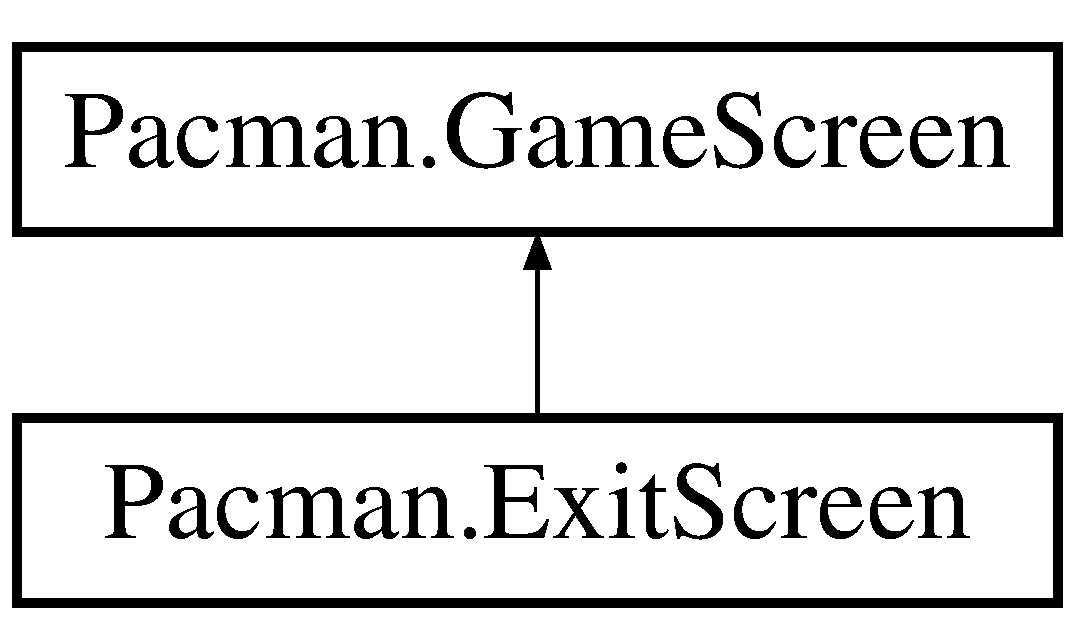
\includegraphics[height=2.000000cm]{class_pacman_1_1_exit_screen}
\end{center}
\end{figure}
\subsection*{Public Member Functions}
\begin{DoxyCompactItemize}
\item 
override bool \hyperlink{class_pacman_1_1_exit_screen_a4177058f3accaa1a45c4ca9599952b16}{Exit} ()
\begin{DoxyCompactList}\small\item\em Only function, returns a true value since we want to close the program \end{DoxyCompactList}\end{DoxyCompactItemize}
\subsection*{Additional Inherited Members}


\subsection{Detailed Description}
Simple screen class that is called when we want to close the program 



\subsection{Member Function Documentation}
\hypertarget{class_pacman_1_1_exit_screen_a4177058f3accaa1a45c4ca9599952b16}{\index{Pacman\-::\-Exit\-Screen@{Pacman\-::\-Exit\-Screen}!Exit@{Exit}}
\index{Exit@{Exit}!Pacman::ExitScreen@{Pacman\-::\-Exit\-Screen}}
\subsubsection[{Exit}]{\setlength{\rightskip}{0pt plus 5cm}override bool Pacman.\-Exit\-Screen.\-Exit (
\begin{DoxyParamCaption}
{}
\end{DoxyParamCaption}
)\hspace{0.3cm}{\ttfamily [virtual]}}}\label{class_pacman_1_1_exit_screen_a4177058f3accaa1a45c4ca9599952b16}


Only function, returns a true value since we want to close the program 

\begin{DoxyReturn}{Returns}

\end{DoxyReturn}


Reimplemented from \hyperlink{class_pacman_1_1_game_screen_a23069d276b1952ecf9fed07d0424e771}{Pacman.\-Game\-Screen}.



The documentation for this class was generated from the following file\-:\begin{DoxyCompactItemize}
\item 
Exit\-Screen.\-cs\end{DoxyCompactItemize}

\hypertarget{class_pacman_1_1_fade_animation}{\section{Pacman.\-Fade\-Animation Class Reference}
\label{class_pacman_1_1_fade_animation}\index{Pacman.\-Fade\-Animation@{Pacman.\-Fade\-Animation}}
}


A fade animation class that fades in and out a image or text, usable for screentransitions  


Inheritance diagram for Pacman.\-Fade\-Animation\-:\begin{figure}[H]
\begin{center}
\leavevmode
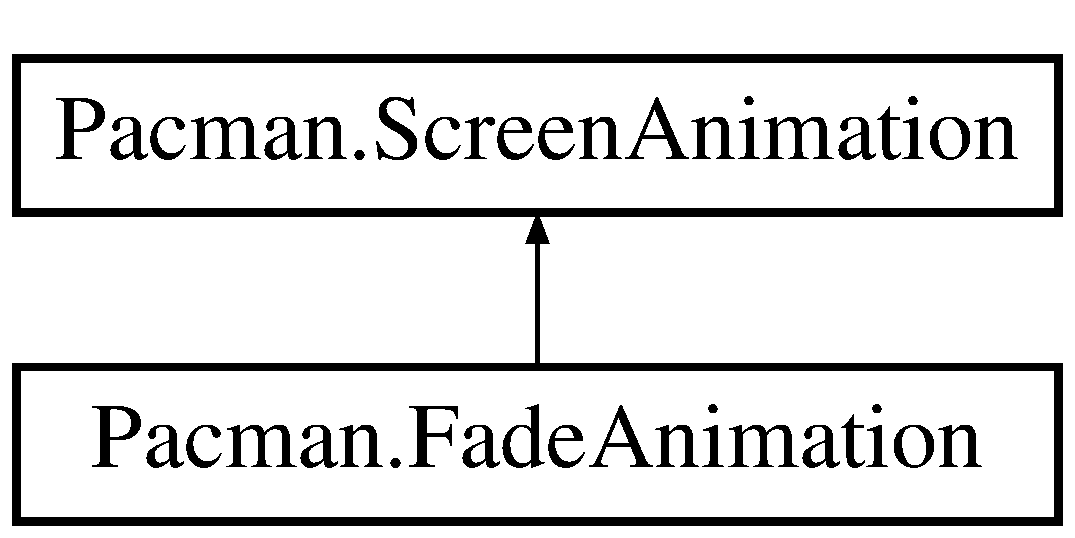
\includegraphics[height=2.000000cm]{class_pacman_1_1_fade_animation}
\end{center}
\end{figure}
\subsection*{Public Member Functions}
\begin{DoxyCompactItemize}
\item 
override void \hyperlink{class_pacman_1_1_fade_animation_a6abddfcfb03a31152da73b6766e99a9d}{Load\-Content} (Content\-Manager Content, Texture2\-D image, string text, Vector2 position, string font\-I\-D)
\begin{DoxyCompactList}\small\item\em Loads in a image, a text string the position in which we want these elements to be drawn on, and the font for the text. sets the default timespan variable to 1 milisecond \end{DoxyCompactList}\item 
override void \hyperlink{class_pacman_1_1_fade_animation_ac6d7c4a5845a19f47dd2501271ecee7a}{Update} (Game\-Time game\-Time)
\begin{DoxyCompactList}\small\item\em Changes the alpha channel value, the value that determines transparency. Fades in or out depending on the increase boolean value. \end{DoxyCompactList}\end{DoxyCompactItemize}
\subsection*{Properties}
\begin{DoxyCompactItemize}
\item 
Time\-Span \hyperlink{class_pacman_1_1_fade_animation_aa161d233c498500c1abc81b15206a53f}{Timer}\hspace{0.3cm}{\ttfamily  \mbox{[}get, set\mbox{]}}
\begin{DoxyCompactList}\small\item\em \hyperlink{class_pacman_1_1_fade_animation}{Fade\-Animation} properties \end{DoxyCompactList}\item 
\hypertarget{class_pacman_1_1_fade_animation_a80295aab2269c152236429d7c210536e}{float {\bfseries Fade\-Speed}\hspace{0.3cm}{\ttfamily  \mbox{[}get, set\mbox{]}}}\label{class_pacman_1_1_fade_animation_a80295aab2269c152236429d7c210536e}

\item 
\hypertarget{class_pacman_1_1_fade_animation_a45fb930d0fb229056d7c534c54b8af86}{override float {\bfseries Alpha}\hspace{0.3cm}{\ttfamily  \mbox{[}get, set\mbox{]}}}\label{class_pacman_1_1_fade_animation_a45fb930d0fb229056d7c534c54b8af86}

\item 
\hypertarget{class_pacman_1_1_fade_animation_a48ffd9f40659312bd0e0de0c3d87b5eb}{float {\bfseries Activate\-Value}\hspace{0.3cm}{\ttfamily  \mbox{[}get, set\mbox{]}}}\label{class_pacman_1_1_fade_animation_a48ffd9f40659312bd0e0de0c3d87b5eb}

\item 
\hypertarget{class_pacman_1_1_fade_animation_a5a828671b9aae1da7d331d995244891f}{bool {\bfseries Increase}\hspace{0.3cm}{\ttfamily  \mbox{[}set\mbox{]}}}\label{class_pacman_1_1_fade_animation_a5a828671b9aae1da7d331d995244891f}

\end{DoxyCompactItemize}
\subsection*{Additional Inherited Members}


\subsection{Detailed Description}
A fade animation class that fades in and out a image or text, usable for screentransitions 



\subsection{Member Function Documentation}
\hypertarget{class_pacman_1_1_fade_animation_a6abddfcfb03a31152da73b6766e99a9d}{\index{Pacman\-::\-Fade\-Animation@{Pacman\-::\-Fade\-Animation}!Load\-Content@{Load\-Content}}
\index{Load\-Content@{Load\-Content}!Pacman::FadeAnimation@{Pacman\-::\-Fade\-Animation}}
\subsubsection[{Load\-Content}]{\setlength{\rightskip}{0pt plus 5cm}override void Pacman.\-Fade\-Animation.\-Load\-Content (
\begin{DoxyParamCaption}
\item[{Content\-Manager}]{Content, }
\item[{Texture2\-D}]{image, }
\item[{string}]{text, }
\item[{Vector2}]{position, }
\item[{string}]{font\-I\-D}
\end{DoxyParamCaption}
)\hspace{0.3cm}{\ttfamily [virtual]}}}\label{class_pacman_1_1_fade_animation_a6abddfcfb03a31152da73b6766e99a9d}


Loads in a image, a text string the position in which we want these elements to be drawn on, and the font for the text. sets the default timespan variable to 1 milisecond 


\begin{DoxyParams}{Parameters}
{\em Content} & \\
\hline
{\em image} & \\
\hline
{\em text} & \\
\hline
{\em position} & \\
\hline
{\em font\-I\-D} & \\
\hline
\end{DoxyParams}


Reimplemented from \hyperlink{class_pacman_1_1_screen_animation_a566ecb3dca9f82c4eb51f4e3a4019550}{Pacman.\-Screen\-Animation}.

\hypertarget{class_pacman_1_1_fade_animation_ac6d7c4a5845a19f47dd2501271ecee7a}{\index{Pacman\-::\-Fade\-Animation@{Pacman\-::\-Fade\-Animation}!Update@{Update}}
\index{Update@{Update}!Pacman::FadeAnimation@{Pacman\-::\-Fade\-Animation}}
\subsubsection[{Update}]{\setlength{\rightskip}{0pt plus 5cm}override void Pacman.\-Fade\-Animation.\-Update (
\begin{DoxyParamCaption}
\item[{Game\-Time}]{game\-Time}
\end{DoxyParamCaption}
)\hspace{0.3cm}{\ttfamily [virtual]}}}\label{class_pacman_1_1_fade_animation_ac6d7c4a5845a19f47dd2501271ecee7a}


Changes the alpha channel value, the value that determines transparency. Fades in or out depending on the increase boolean value. 


\begin{DoxyParams}{Parameters}
{\em game\-Time} & \\
\hline
\end{DoxyParams}


Reimplemented from \hyperlink{class_pacman_1_1_screen_animation_af381913622005dfb6b759f7495b37ded}{Pacman.\-Screen\-Animation}.



\subsection{Property Documentation}
\hypertarget{class_pacman_1_1_fade_animation_aa161d233c498500c1abc81b15206a53f}{\index{Pacman\-::\-Fade\-Animation@{Pacman\-::\-Fade\-Animation}!Timer@{Timer}}
\index{Timer@{Timer}!Pacman::FadeAnimation@{Pacman\-::\-Fade\-Animation}}
\subsubsection[{Timer}]{\setlength{\rightskip}{0pt plus 5cm}Time\-Span Pacman.\-Fade\-Animation.\-Timer\hspace{0.3cm}{\ttfamily [get]}, {\ttfamily [set]}}}\label{class_pacman_1_1_fade_animation_aa161d233c498500c1abc81b15206a53f}


\hyperlink{class_pacman_1_1_fade_animation}{Fade\-Animation} properties 



The documentation for this class was generated from the following file\-:\begin{DoxyCompactItemize}
\item 
Fade\-Animation.\-cs\end{DoxyCompactItemize}

\hypertarget{class_pacman_1_1_file_manager}{\section{Pacman.\-File\-Manager Class Reference}
\label{class_pacman_1_1_file_manager}\index{Pacman.\-File\-Manager@{Pacman.\-File\-Manager}}
}


A filemanager class that helps reading and writing elements to/from a file to the program. Uses both normal text files and X\-M\-L files  


\subsection*{Public Member Functions}
\begin{DoxyCompactItemize}
\item 
void \hyperlink{class_pacman_1_1_file_manager_a4a5be095e8de90a583f3f99ac89300ff}{Load\-Content} (string filename, List$<$ List$<$ string $>$$>$ attributes, List$<$ List$<$ string $>$$>$ contents)
\begin{DoxyCompactList}\small\item\em Reads everything from a specified text file, the file has to be formatted for the specific function or it will not be read properly. Puts in the read data onto the two, two dimensional Lists. Attributes is the identifyer telling what type of data that is being loaded in. Contents is the actual data. \end{DoxyCompactList}\item 
void \hyperlink{class_pacman_1_1_file_manager_af3b152657eefb8f967dbdd2edca6c7dd}{Load\-Content} (string filename, List$<$ List$<$ string $>$$>$ attributes, List$<$ List$<$ string $>$$>$ contents, string identifier)
\begin{DoxyCompactList}\small\item\em An overloaded version of the Load\-Content that starts to read when the identifier requirments are met and stops reading when told to. Other then that it does the same as the first Load\-Content. \end{DoxyCompactList}\item 
void \hyperlink{class_pacman_1_1_file_manager_a00288173f2ae8a7957797c553b00d760}{Read\-Score} (string file\-Name, List$<$ int $>$ score, List$<$ string $>$ player\-Name)
\begin{DoxyCompactList}\small\item\em Reads the score from a X\-M\-L file, puts the name and score in their respective list. \end{DoxyCompactList}\item 
void \hyperlink{class_pacman_1_1_file_manager_aedf31e50cc3f1f7aba5566e324d139ef}{Write\-Score} (string file\-Name, int player\-Score, string player\-Name)
\begin{DoxyCompactList}\small\item\em Appends the score and name to a X\-M\-L file \end{DoxyCompactList}\end{DoxyCompactItemize}


\subsection{Detailed Description}
A filemanager class that helps reading and writing elements to/from a file to the program. Uses both normal text files and X\-M\-L files 



\subsection{Member Function Documentation}
\hypertarget{class_pacman_1_1_file_manager_a4a5be095e8de90a583f3f99ac89300ff}{\index{Pacman\-::\-File\-Manager@{Pacman\-::\-File\-Manager}!Load\-Content@{Load\-Content}}
\index{Load\-Content@{Load\-Content}!Pacman::FileManager@{Pacman\-::\-File\-Manager}}
\subsubsection[{Load\-Content}]{\setlength{\rightskip}{0pt plus 5cm}void Pacman.\-File\-Manager.\-Load\-Content (
\begin{DoxyParamCaption}
\item[{string}]{filename, }
\item[{List$<$ List$<$ string $>$$>$}]{attributes, }
\item[{List$<$ List$<$ string $>$$>$}]{contents}
\end{DoxyParamCaption}
)}}\label{class_pacman_1_1_file_manager_a4a5be095e8de90a583f3f99ac89300ff}


Reads everything from a specified text file, the file has to be formatted for the specific function or it will not be read properly. Puts in the read data onto the two, two dimensional Lists. Attributes is the identifyer telling what type of data that is being loaded in. Contents is the actual data. 


\begin{DoxyParams}{Parameters}
{\em filename} & \\
\hline
{\em attributes} & \\
\hline
{\em contents} & \\
\hline
\end{DoxyParams}
\hypertarget{class_pacman_1_1_file_manager_af3b152657eefb8f967dbdd2edca6c7dd}{\index{Pacman\-::\-File\-Manager@{Pacman\-::\-File\-Manager}!Load\-Content@{Load\-Content}}
\index{Load\-Content@{Load\-Content}!Pacman::FileManager@{Pacman\-::\-File\-Manager}}
\subsubsection[{Load\-Content}]{\setlength{\rightskip}{0pt plus 5cm}void Pacman.\-File\-Manager.\-Load\-Content (
\begin{DoxyParamCaption}
\item[{string}]{filename, }
\item[{List$<$ List$<$ string $>$$>$}]{attributes, }
\item[{List$<$ List$<$ string $>$$>$}]{contents, }
\item[{string}]{identifier}
\end{DoxyParamCaption}
)}}\label{class_pacman_1_1_file_manager_af3b152657eefb8f967dbdd2edca6c7dd}


An overloaded version of the Load\-Content that starts to read when the identifier requirments are met and stops reading when told to. Other then that it does the same as the first Load\-Content. 


\begin{DoxyParams}{Parameters}
{\em filename} & \\
\hline
{\em attributes} & \\
\hline
{\em contents} & \\
\hline
{\em identifier} & \\
\hline
\end{DoxyParams}
\hypertarget{class_pacman_1_1_file_manager_a00288173f2ae8a7957797c553b00d760}{\index{Pacman\-::\-File\-Manager@{Pacman\-::\-File\-Manager}!Read\-Score@{Read\-Score}}
\index{Read\-Score@{Read\-Score}!Pacman::FileManager@{Pacman\-::\-File\-Manager}}
\subsubsection[{Read\-Score}]{\setlength{\rightskip}{0pt plus 5cm}void Pacman.\-File\-Manager.\-Read\-Score (
\begin{DoxyParamCaption}
\item[{string}]{file\-Name, }
\item[{List$<$ int $>$}]{score, }
\item[{List$<$ string $>$}]{player\-Name}
\end{DoxyParamCaption}
)}}\label{class_pacman_1_1_file_manager_a00288173f2ae8a7957797c553b00d760}


Reads the score from a X\-M\-L file, puts the name and score in their respective list. 


\begin{DoxyParams}{Parameters}
{\em file\-Name} & \\
\hline
{\em score} & \\
\hline
{\em player\-Name} & \\
\hline
\end{DoxyParams}
\hypertarget{class_pacman_1_1_file_manager_aedf31e50cc3f1f7aba5566e324d139ef}{\index{Pacman\-::\-File\-Manager@{Pacman\-::\-File\-Manager}!Write\-Score@{Write\-Score}}
\index{Write\-Score@{Write\-Score}!Pacman::FileManager@{Pacman\-::\-File\-Manager}}
\subsubsection[{Write\-Score}]{\setlength{\rightskip}{0pt plus 5cm}void Pacman.\-File\-Manager.\-Write\-Score (
\begin{DoxyParamCaption}
\item[{string}]{file\-Name, }
\item[{int}]{player\-Score, }
\item[{string}]{player\-Name}
\end{DoxyParamCaption}
)}}\label{class_pacman_1_1_file_manager_aedf31e50cc3f1f7aba5566e324d139ef}


Appends the score and name to a X\-M\-L file 


\begin{DoxyParams}{Parameters}
{\em file\-Name} & \\
\hline
{\em player\-Score} & \\
\hline
{\em player\-Name} & \\
\hline
\end{DoxyParams}


The documentation for this class was generated from the following file\-:\begin{DoxyCompactItemize}
\item 
File\-Manager.\-cs\end{DoxyCompactItemize}

\hypertarget{class_pacman_1_1_game1}{\section{Pacman.\-Game1 Class Reference}
\label{class_pacman_1_1_game1}\index{Pacman.\-Game1@{Pacman.\-Game1}}
}


This is the main type for your game  


Inheritance diagram for Pacman.\-Game1\-:\begin{figure}[H]
\begin{center}
\leavevmode
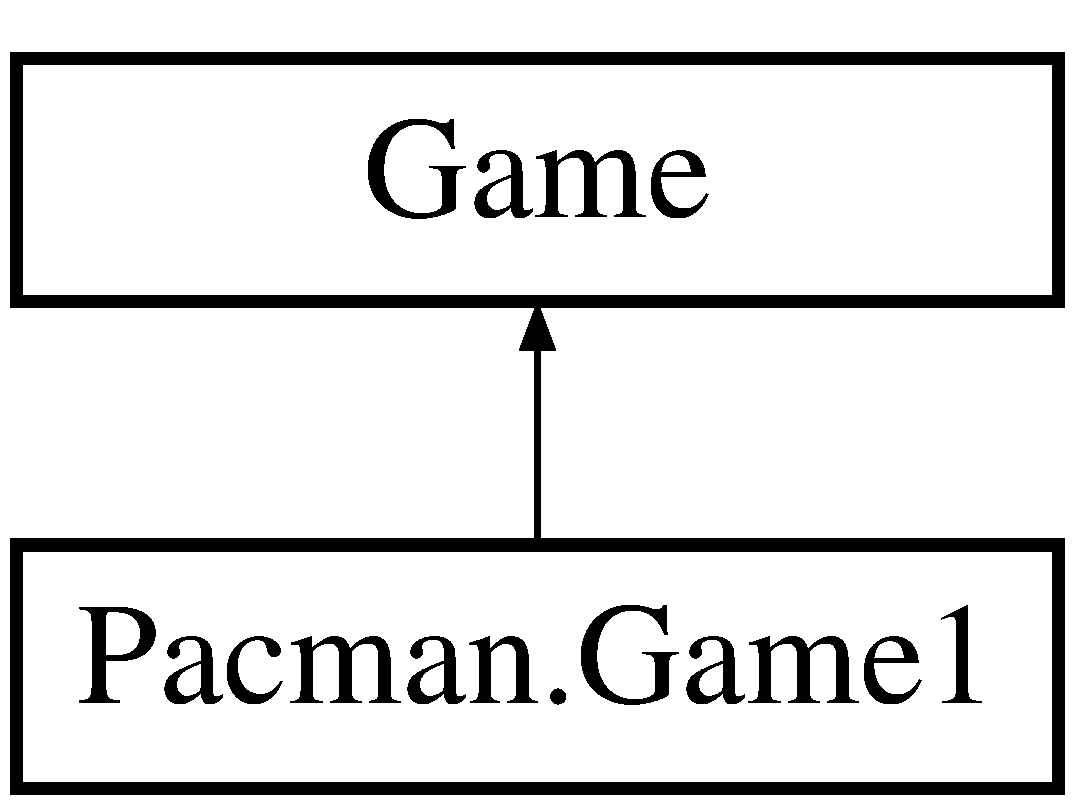
\includegraphics[height=2.000000cm]{class_pacman_1_1_game1}
\end{center}
\end{figure}
\subsection*{Public Member Functions}
\begin{DoxyCompactItemize}
\item 
\hypertarget{class_pacman_1_1_game1_a06dfb68d52150fb8f15f7d739947b7ac}{{\bfseries Game1} (bool exit)}\label{class_pacman_1_1_game1_a06dfb68d52150fb8f15f7d739947b7ac}

\end{DoxyCompactItemize}
\subsection*{Protected Member Functions}
\begin{DoxyCompactItemize}
\item 
override void \hyperlink{class_pacman_1_1_game1_a55a2bc52a62f5813f20860d10d7614f5}{Initialize} ()
\begin{DoxyCompactList}\small\item\em Initializes the \hyperlink{class_pacman_1_1_screen_manager}{Screen\-Manager}, sets the dimensions of the game window \end{DoxyCompactList}\item 
override void \hyperlink{class_pacman_1_1_game1_a9c5fd4623bf1d9d6b1ea2cb37e5f2b3a}{Load\-Content} ()
\begin{DoxyCompactList}\small\item\em Gives the \hyperlink{class_pacman_1_1_screen_manager}{Screen\-Manager} class it's own Contentmanager \end{DoxyCompactList}\item 
\hypertarget{class_pacman_1_1_game1_a5742bbddb5003b69c5068dd9ea632a78}{override void {\bfseries Unload\-Content} ()}\label{class_pacman_1_1_game1_a5742bbddb5003b69c5068dd9ea632a78}

\item 
override void \hyperlink{class_pacman_1_1_game1_a8d7c660a92475d021af8e2da33f0af1b}{Update} (Game\-Time game\-Time)
\begin{DoxyCompactList}\small\item\em Checks to see if we want to exit if not then update the current screen \end{DoxyCompactList}\item 
override void \hyperlink{class_pacman_1_1_game1_aa296bdd57b2e540aebc8ab81c9f166a4}{Draw} (Game\-Time game\-Time)
\begin{DoxyCompactList}\small\item\em Draw the current screen \end{DoxyCompactList}\end{DoxyCompactItemize}


\subsection{Detailed Description}
This is the main type for your game 



\subsection{Member Function Documentation}
\hypertarget{class_pacman_1_1_game1_aa296bdd57b2e540aebc8ab81c9f166a4}{\index{Pacman\-::\-Game1@{Pacman\-::\-Game1}!Draw@{Draw}}
\index{Draw@{Draw}!Pacman::Game1@{Pacman\-::\-Game1}}
\subsubsection[{Draw}]{\setlength{\rightskip}{0pt plus 5cm}override void Pacman.\-Game1.\-Draw (
\begin{DoxyParamCaption}
\item[{Game\-Time}]{game\-Time}
\end{DoxyParamCaption}
)\hspace{0.3cm}{\ttfamily [protected]}}}\label{class_pacman_1_1_game1_aa296bdd57b2e540aebc8ab81c9f166a4}


Draw the current screen 


\begin{DoxyParams}{Parameters}
{\em game\-Time} & \\
\hline
\end{DoxyParams}
\hypertarget{class_pacman_1_1_game1_a55a2bc52a62f5813f20860d10d7614f5}{\index{Pacman\-::\-Game1@{Pacman\-::\-Game1}!Initialize@{Initialize}}
\index{Initialize@{Initialize}!Pacman::Game1@{Pacman\-::\-Game1}}
\subsubsection[{Initialize}]{\setlength{\rightskip}{0pt plus 5cm}override void Pacman.\-Game1.\-Initialize (
\begin{DoxyParamCaption}
{}
\end{DoxyParamCaption}
)\hspace{0.3cm}{\ttfamily [protected]}}}\label{class_pacman_1_1_game1_a55a2bc52a62f5813f20860d10d7614f5}


Initializes the \hyperlink{class_pacman_1_1_screen_manager}{Screen\-Manager}, sets the dimensions of the game window 

\hypertarget{class_pacman_1_1_game1_a9c5fd4623bf1d9d6b1ea2cb37e5f2b3a}{\index{Pacman\-::\-Game1@{Pacman\-::\-Game1}!Load\-Content@{Load\-Content}}
\index{Load\-Content@{Load\-Content}!Pacman::Game1@{Pacman\-::\-Game1}}
\subsubsection[{Load\-Content}]{\setlength{\rightskip}{0pt plus 5cm}override void Pacman.\-Game1.\-Load\-Content (
\begin{DoxyParamCaption}
{}
\end{DoxyParamCaption}
)\hspace{0.3cm}{\ttfamily [protected]}}}\label{class_pacman_1_1_game1_a9c5fd4623bf1d9d6b1ea2cb37e5f2b3a}


Gives the \hyperlink{class_pacman_1_1_screen_manager}{Screen\-Manager} class it's own Contentmanager 

\hypertarget{class_pacman_1_1_game1_a8d7c660a92475d021af8e2da33f0af1b}{\index{Pacman\-::\-Game1@{Pacman\-::\-Game1}!Update@{Update}}
\index{Update@{Update}!Pacman::Game1@{Pacman\-::\-Game1}}
\subsubsection[{Update}]{\setlength{\rightskip}{0pt plus 5cm}override void Pacman.\-Game1.\-Update (
\begin{DoxyParamCaption}
\item[{Game\-Time}]{game\-Time}
\end{DoxyParamCaption}
)\hspace{0.3cm}{\ttfamily [protected]}}}\label{class_pacman_1_1_game1_a8d7c660a92475d021af8e2da33f0af1b}


Checks to see if we want to exit if not then update the current screen 


\begin{DoxyParams}{Parameters}
{\em game\-Time} & \\
\hline
\end{DoxyParams}


The documentation for this class was generated from the following file\-:\begin{DoxyCompactItemize}
\item 
Game1.\-cs\end{DoxyCompactItemize}

\hypertarget{class_pacman_1_1_game_over}{\section{Pacman.\-Game\-Over Class Reference}
\label{class_pacman_1_1_game_over}\index{Pacman.\-Game\-Over@{Pacman.\-Game\-Over}}
}


Class that checks if a gameover criteria has been met.  


\subsection*{Public Member Functions}
\begin{DoxyCompactItemize}
\item 
bool \hyperlink{class_pacman_1_1_game_over_a8c6e6a54940e95d859ee8fe53deb5d00}{Check\-Game\-State} (\hyperlink{class_pacman_1_1_player}{Player} player, \hyperlink{class_pacman_1_1_enemy}{Enemy} enemy, \hyperlink{class_pacman_1_1_layers}{Layers} layer)
\begin{DoxyCompactList}\small\item\em calls the two private mathods and return a true if the citeria has been met or false if not \end{DoxyCompactList}\end{DoxyCompactItemize}


\subsection{Detailed Description}
Class that checks if a gameover criteria has been met. 



\subsection{Member Function Documentation}
\hypertarget{class_pacman_1_1_game_over_a8c6e6a54940e95d859ee8fe53deb5d00}{\index{Pacman\-::\-Game\-Over@{Pacman\-::\-Game\-Over}!Check\-Game\-State@{Check\-Game\-State}}
\index{Check\-Game\-State@{Check\-Game\-State}!Pacman::GameOver@{Pacman\-::\-Game\-Over}}
\subsubsection[{Check\-Game\-State}]{\setlength{\rightskip}{0pt plus 5cm}bool Pacman.\-Game\-Over.\-Check\-Game\-State (
\begin{DoxyParamCaption}
\item[{{\bf Player}}]{player, }
\item[{{\bf Enemy}}]{enemy, }
\item[{{\bf Layers}}]{layer}
\end{DoxyParamCaption}
)}}\label{class_pacman_1_1_game_over_a8c6e6a54940e95d859ee8fe53deb5d00}


calls the two private mathods and return a true if the citeria has been met or false if not 


\begin{DoxyParams}{Parameters}
{\em player} & \\
\hline
{\em enemy} & \\
\hline
{\em layer} & \\
\hline
\end{DoxyParams}
\begin{DoxyReturn}{Returns}

\end{DoxyReturn}


The documentation for this class was generated from the following file\-:\begin{DoxyCompactItemize}
\item 
Game\-Over.\-cs\end{DoxyCompactItemize}

\hypertarget{class_pacman_1_1_game_over_screen}{\section{Pacman.\-Game\-Over\-Screen Class Reference}
\label{class_pacman_1_1_game_over_screen}\index{Pacman.\-Game\-Over\-Screen@{Pacman.\-Game\-Over\-Screen}}
}


The screen that appears when you lost or won the game  


Inheritance diagram for Pacman.\-Game\-Over\-Screen\-:\begin{figure}[H]
\begin{center}
\leavevmode
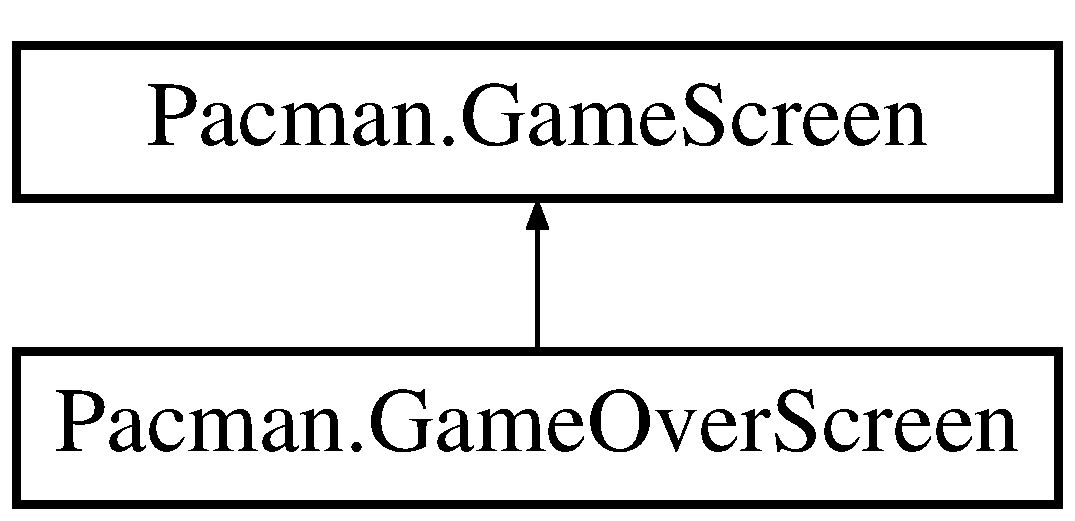
\includegraphics[height=2.000000cm]{class_pacman_1_1_game_over_screen}
\end{center}
\end{figure}
\subsection*{Public Member Functions}
\begin{DoxyCompactItemize}
\item 
\hyperlink{class_pacman_1_1_game_over_screen_a7d97bf9092aecb4d9de8cd93e444f4f1}{Game\-Over\-Screen} (\hyperlink{class_pacman_1_1_high_score}{High\-Score} high\-Score)
\begin{DoxyCompactList}\small\item\em Constructor that gets the current highscore class \end{DoxyCompactList}\item 
override void \hyperlink{class_pacman_1_1_game_over_screen_a43eaf6170505796fcfb0bdb73560c744}{Load\-Content} (Content\-Manager Content)
\begin{DoxyCompactList}\small\item\em Loads in all the fonts, sets the textfade animation to true,and initializes all the variables. \end{DoxyCompactList}\item 
override void \hyperlink{class_pacman_1_1_game_over_screen_a70173a7767450e66a6deeb00bc4a5844}{Unload\-Content} ()
\begin{DoxyCompactList}\small\item\em Unloads the highscore class and the base class, called when a new screen is added \end{DoxyCompactList}\item 
override void \hyperlink{class_pacman_1_1_game_over_screen_abfdcd8b539aa5020bf9e34a86072ae81}{Update} (Game\-Time game\-Time)
\begin{DoxyCompactList}\small\item\em Gets the keyboard input for the player name text input dialog, saves the highscore when eneter is press, the user then also is taken back to the mainmenu by adding a new \hyperlink{class_pacman_1_1_main_menu}{Main\-Menu} screen. \end{DoxyCompactList}\item 
override void \hyperlink{class_pacman_1_1_game_over_screen_ae8e0cb7c8d8f836483c2e0e776e939ef}{Draw} (Sprite\-Batch sprite\-Batch)
\begin{DoxyCompactList}\small\item\em Draws the different texts and inputtext also the textfade animation draw function is called. \end{DoxyCompactList}\end{DoxyCompactItemize}
\subsection*{Additional Inherited Members}


\subsection{Detailed Description}
The screen that appears when you lost or won the game 



\subsection{Constructor \& Destructor Documentation}
\hypertarget{class_pacman_1_1_game_over_screen_a7d97bf9092aecb4d9de8cd93e444f4f1}{\index{Pacman\-::\-Game\-Over\-Screen@{Pacman\-::\-Game\-Over\-Screen}!Game\-Over\-Screen@{Game\-Over\-Screen}}
\index{Game\-Over\-Screen@{Game\-Over\-Screen}!Pacman::GameOverScreen@{Pacman\-::\-Game\-Over\-Screen}}
\subsubsection[{Game\-Over\-Screen}]{\setlength{\rightskip}{0pt plus 5cm}Pacman.\-Game\-Over\-Screen.\-Game\-Over\-Screen (
\begin{DoxyParamCaption}
\item[{{\bf High\-Score}}]{high\-Score}
\end{DoxyParamCaption}
)}}\label{class_pacman_1_1_game_over_screen_a7d97bf9092aecb4d9de8cd93e444f4f1}


Constructor that gets the current highscore class 


\begin{DoxyParams}{Parameters}
{\em high\-Score} & \\
\hline
\end{DoxyParams}


\subsection{Member Function Documentation}
\hypertarget{class_pacman_1_1_game_over_screen_ae8e0cb7c8d8f836483c2e0e776e939ef}{\index{Pacman\-::\-Game\-Over\-Screen@{Pacman\-::\-Game\-Over\-Screen}!Draw@{Draw}}
\index{Draw@{Draw}!Pacman::GameOverScreen@{Pacman\-::\-Game\-Over\-Screen}}
\subsubsection[{Draw}]{\setlength{\rightskip}{0pt plus 5cm}override void Pacman.\-Game\-Over\-Screen.\-Draw (
\begin{DoxyParamCaption}
\item[{Sprite\-Batch}]{sprite\-Batch}
\end{DoxyParamCaption}
)\hspace{0.3cm}{\ttfamily [virtual]}}}\label{class_pacman_1_1_game_over_screen_ae8e0cb7c8d8f836483c2e0e776e939ef}


Draws the different texts and inputtext also the textfade animation draw function is called. 


\begin{DoxyParams}{Parameters}
{\em sprite\-Batch} & \\
\hline
\end{DoxyParams}


Reimplemented from \hyperlink{class_pacman_1_1_game_screen_ab7d62816f246e29e70d352d094c36b04}{Pacman.\-Game\-Screen}.

\hypertarget{class_pacman_1_1_game_over_screen_a43eaf6170505796fcfb0bdb73560c744}{\index{Pacman\-::\-Game\-Over\-Screen@{Pacman\-::\-Game\-Over\-Screen}!Load\-Content@{Load\-Content}}
\index{Load\-Content@{Load\-Content}!Pacman::GameOverScreen@{Pacman\-::\-Game\-Over\-Screen}}
\subsubsection[{Load\-Content}]{\setlength{\rightskip}{0pt plus 5cm}override void Pacman.\-Game\-Over\-Screen.\-Load\-Content (
\begin{DoxyParamCaption}
\item[{Content\-Manager}]{Content}
\end{DoxyParamCaption}
)\hspace{0.3cm}{\ttfamily [virtual]}}}\label{class_pacman_1_1_game_over_screen_a43eaf6170505796fcfb0bdb73560c744}


Loads in all the fonts, sets the textfade animation to true,and initializes all the variables. 


\begin{DoxyParams}{Parameters}
{\em Content} & \\
\hline
\end{DoxyParams}


Reimplemented from \hyperlink{class_pacman_1_1_game_screen_a33dbdc943439ae7728aff62b5152aa53}{Pacman.\-Game\-Screen}.

\hypertarget{class_pacman_1_1_game_over_screen_a70173a7767450e66a6deeb00bc4a5844}{\index{Pacman\-::\-Game\-Over\-Screen@{Pacman\-::\-Game\-Over\-Screen}!Unload\-Content@{Unload\-Content}}
\index{Unload\-Content@{Unload\-Content}!Pacman::GameOverScreen@{Pacman\-::\-Game\-Over\-Screen}}
\subsubsection[{Unload\-Content}]{\setlength{\rightskip}{0pt plus 5cm}override void Pacman.\-Game\-Over\-Screen.\-Unload\-Content (
\begin{DoxyParamCaption}
{}
\end{DoxyParamCaption}
)\hspace{0.3cm}{\ttfamily [virtual]}}}\label{class_pacman_1_1_game_over_screen_a70173a7767450e66a6deeb00bc4a5844}


Unloads the highscore class and the base class, called when a new screen is added 



Reimplemented from \hyperlink{class_pacman_1_1_game_screen_aa33ba4650a38762eca4bd059fb803942}{Pacman.\-Game\-Screen}.

\hypertarget{class_pacman_1_1_game_over_screen_abfdcd8b539aa5020bf9e34a86072ae81}{\index{Pacman\-::\-Game\-Over\-Screen@{Pacman\-::\-Game\-Over\-Screen}!Update@{Update}}
\index{Update@{Update}!Pacman::GameOverScreen@{Pacman\-::\-Game\-Over\-Screen}}
\subsubsection[{Update}]{\setlength{\rightskip}{0pt plus 5cm}override void Pacman.\-Game\-Over\-Screen.\-Update (
\begin{DoxyParamCaption}
\item[{Game\-Time}]{game\-Time}
\end{DoxyParamCaption}
)\hspace{0.3cm}{\ttfamily [virtual]}}}\label{class_pacman_1_1_game_over_screen_abfdcd8b539aa5020bf9e34a86072ae81}


Gets the keyboard input for the player name text input dialog, saves the highscore when eneter is press, the user then also is taken back to the mainmenu by adding a new \hyperlink{class_pacman_1_1_main_menu}{Main\-Menu} screen. 


\begin{DoxyParams}{Parameters}
{\em game\-Time} & \\
\hline
\end{DoxyParams}


Reimplemented from \hyperlink{class_pacman_1_1_game_screen_a768b26cbc3ed823d0dcba5055ae9a8b4}{Pacman.\-Game\-Screen}.



The documentation for this class was generated from the following file\-:\begin{DoxyCompactItemize}
\item 
Game\-Over\-Screen.\-cs\end{DoxyCompactItemize}

\hypertarget{class_pacman_1_1_game_screen}{\section{Pacman.\-Game\-Screen Class Reference}
\label{class_pacman_1_1_game_screen}\index{Pacman.\-Game\-Screen@{Pacman.\-Game\-Screen}}
}


The base class of all the different screens  


Inheritance diagram for Pacman.\-Game\-Screen\-:\begin{figure}[H]
\begin{center}
\leavevmode
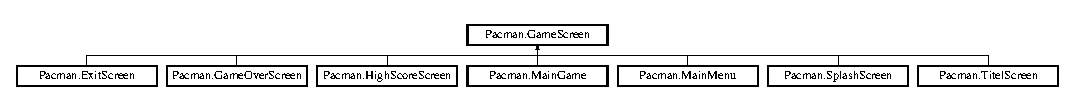
\includegraphics[height=0.935673cm]{class_pacman_1_1_game_screen}
\end{center}
\end{figure}
\subsection*{Public Member Functions}
\begin{DoxyCompactItemize}
\item 
virtual void \hyperlink{class_pacman_1_1_game_screen_aa33ba4650a38762eca4bd059fb803942}{Unload\-Content} ()
\begin{DoxyCompactList}\small\item\em Unloads the contentmanager \end{DoxyCompactList}\item 
virtual void \hyperlink{class_pacman_1_1_game_screen_a33dbdc943439ae7728aff62b5152aa53}{Load\-Content} (Content\-Manager Content)
\begin{DoxyCompactList}\small\item\em Loads the contentmanager to the one that \hyperlink{class_pacman_1_1_game1}{Game1} is using. initializes the lists \end{DoxyCompactList}\item 
virtual void \hyperlink{class_pacman_1_1_game_screen_a768b26cbc3ed823d0dcba5055ae9a8b4}{Update} (Game\-Time game\-Time)
\begin{DoxyCompactList}\small\item\em Generic update funcion \end{DoxyCompactList}\item 
virtual void \hyperlink{class_pacman_1_1_game_screen_ab7d62816f246e29e70d352d094c36b04}{Draw} (Sprite\-Batch sprite\-Batch)
\begin{DoxyCompactList}\small\item\em Generic draw function \end{DoxyCompactList}\item 
virtual bool \hyperlink{class_pacman_1_1_game_screen_a23069d276b1952ecf9fed07d0424e771}{Exit} ()
\begin{DoxyCompactList}\small\item\em Allways returns false except when changed. \end{DoxyCompactList}\end{DoxyCompactItemize}
\subsection*{Protected Attributes}
\begin{DoxyCompactItemize}
\item 
\hypertarget{class_pacman_1_1_game_screen_a89f510b4d354e6b1eb68b41b108e3ffd}{Content\-Manager {\bfseries content}}\label{class_pacman_1_1_game_screen_a89f510b4d354e6b1eb68b41b108e3ffd}

\item 
\hypertarget{class_pacman_1_1_game_screen_aae34556caa8e4fd97aa4f639f08785c4}{List$<$ List$<$ string $>$ $>$ {\bfseries attributes}}\label{class_pacman_1_1_game_screen_aae34556caa8e4fd97aa4f639f08785c4}

\end{DoxyCompactItemize}


\subsection{Detailed Description}
The base class of all the different screens 



\subsection{Member Function Documentation}
\hypertarget{class_pacman_1_1_game_screen_ab7d62816f246e29e70d352d094c36b04}{\index{Pacman\-::\-Game\-Screen@{Pacman\-::\-Game\-Screen}!Draw@{Draw}}
\index{Draw@{Draw}!Pacman::GameScreen@{Pacman\-::\-Game\-Screen}}
\subsubsection[{Draw}]{\setlength{\rightskip}{0pt plus 5cm}virtual void Pacman.\-Game\-Screen.\-Draw (
\begin{DoxyParamCaption}
\item[{Sprite\-Batch}]{sprite\-Batch}
\end{DoxyParamCaption}
)\hspace{0.3cm}{\ttfamily [virtual]}}}\label{class_pacman_1_1_game_screen_ab7d62816f246e29e70d352d094c36b04}


Generic draw function 


\begin{DoxyParams}{Parameters}
{\em sprite\-Batch} & \\
\hline
\end{DoxyParams}


Reimplemented in \hyperlink{class_pacman_1_1_game_over_screen_ae8e0cb7c8d8f836483c2e0e776e939ef}{Pacman.\-Game\-Over\-Screen}, \hyperlink{class_pacman_1_1_splash_screen_a669ad3120d15e6eea2636e44d74cdc31}{Pacman.\-Splash\-Screen}, \hyperlink{class_pacman_1_1_main_game_ae0723e8c7fcc6fe57383774b84bc5c91}{Pacman.\-Main\-Game}, \hyperlink{class_pacman_1_1_titel_screen_ae86c21742cdd405fd4467b67b509bc6d}{Pacman.\-Titel\-Screen}, \hyperlink{class_pacman_1_1_high_score_screen_ad785f3290cea4ce2483d89dd651bee76}{Pacman.\-High\-Score\-Screen}, and \hyperlink{class_pacman_1_1_main_menu_aa1ea98563a955497e06808b440a65712}{Pacman.\-Main\-Menu}.

\hypertarget{class_pacman_1_1_game_screen_a23069d276b1952ecf9fed07d0424e771}{\index{Pacman\-::\-Game\-Screen@{Pacman\-::\-Game\-Screen}!Exit@{Exit}}
\index{Exit@{Exit}!Pacman::GameScreen@{Pacman\-::\-Game\-Screen}}
\subsubsection[{Exit}]{\setlength{\rightskip}{0pt plus 5cm}virtual bool Pacman.\-Game\-Screen.\-Exit (
\begin{DoxyParamCaption}
{}
\end{DoxyParamCaption}
)\hspace{0.3cm}{\ttfamily [virtual]}}}\label{class_pacman_1_1_game_screen_a23069d276b1952ecf9fed07d0424e771}


Allways returns false except when changed. 

\begin{DoxyReturn}{Returns}

\end{DoxyReturn}


Reimplemented in \hyperlink{class_pacman_1_1_exit_screen_a4177058f3accaa1a45c4ca9599952b16}{Pacman.\-Exit\-Screen}.

\hypertarget{class_pacman_1_1_game_screen_a33dbdc943439ae7728aff62b5152aa53}{\index{Pacman\-::\-Game\-Screen@{Pacman\-::\-Game\-Screen}!Load\-Content@{Load\-Content}}
\index{Load\-Content@{Load\-Content}!Pacman::GameScreen@{Pacman\-::\-Game\-Screen}}
\subsubsection[{Load\-Content}]{\setlength{\rightskip}{0pt plus 5cm}virtual void Pacman.\-Game\-Screen.\-Load\-Content (
\begin{DoxyParamCaption}
\item[{Content\-Manager}]{Content}
\end{DoxyParamCaption}
)\hspace{0.3cm}{\ttfamily [virtual]}}}\label{class_pacman_1_1_game_screen_a33dbdc943439ae7728aff62b5152aa53}


Loads the contentmanager to the one that \hyperlink{class_pacman_1_1_game1}{Game1} is using. initializes the lists 


\begin{DoxyParams}{Parameters}
{\em Content} & \\
\hline
\end{DoxyParams}


Reimplemented in \hyperlink{class_pacman_1_1_game_over_screen_a43eaf6170505796fcfb0bdb73560c744}{Pacman.\-Game\-Over\-Screen}, \hyperlink{class_pacman_1_1_splash_screen_a05a5f91c7e0ded6cb4893da9eeb0ded1}{Pacman.\-Splash\-Screen}, \hyperlink{class_pacman_1_1_main_game_a8d51b2ec6cc93f142309ea6fe36b2b30}{Pacman.\-Main\-Game}, \hyperlink{class_pacman_1_1_titel_screen_aaeeb7b4a31657e20e6d37926d38e5c31}{Pacman.\-Titel\-Screen}, \hyperlink{class_pacman_1_1_high_score_screen_a2f9c7bd488af9db87c5e74c5e4d21a4e}{Pacman.\-High\-Score\-Screen}, and \hyperlink{class_pacman_1_1_main_menu_afe334b467dd04341970f6a37521afbd5}{Pacman.\-Main\-Menu}.

\hypertarget{class_pacman_1_1_game_screen_aa33ba4650a38762eca4bd059fb803942}{\index{Pacman\-::\-Game\-Screen@{Pacman\-::\-Game\-Screen}!Unload\-Content@{Unload\-Content}}
\index{Unload\-Content@{Unload\-Content}!Pacman::GameScreen@{Pacman\-::\-Game\-Screen}}
\subsubsection[{Unload\-Content}]{\setlength{\rightskip}{0pt plus 5cm}virtual void Pacman.\-Game\-Screen.\-Unload\-Content (
\begin{DoxyParamCaption}
{}
\end{DoxyParamCaption}
)\hspace{0.3cm}{\ttfamily [virtual]}}}\label{class_pacman_1_1_game_screen_aa33ba4650a38762eca4bd059fb803942}


Unloads the contentmanager 



Reimplemented in \hyperlink{class_pacman_1_1_main_game_a7858b061a1db731df54381e03f71b7e0}{Pacman.\-Main\-Game}, \hyperlink{class_pacman_1_1_splash_screen_ac72328daa3003fa228218c65660c8d6c}{Pacman.\-Splash\-Screen}, \hyperlink{class_pacman_1_1_game_over_screen_a70173a7767450e66a6deeb00bc4a5844}{Pacman.\-Game\-Over\-Screen}, \hyperlink{class_pacman_1_1_titel_screen_ae9feed8a91c5fe3da560994fe4258fb2}{Pacman.\-Titel\-Screen}, \hyperlink{class_pacman_1_1_high_score_screen_a9486bf7d1079734d5cf842b53c8f4ade}{Pacman.\-High\-Score\-Screen}, and \hyperlink{class_pacman_1_1_main_menu_a5081e962db4976366a69d7e762680edd}{Pacman.\-Main\-Menu}.

\hypertarget{class_pacman_1_1_game_screen_a768b26cbc3ed823d0dcba5055ae9a8b4}{\index{Pacman\-::\-Game\-Screen@{Pacman\-::\-Game\-Screen}!Update@{Update}}
\index{Update@{Update}!Pacman::GameScreen@{Pacman\-::\-Game\-Screen}}
\subsubsection[{Update}]{\setlength{\rightskip}{0pt plus 5cm}virtual void Pacman.\-Game\-Screen.\-Update (
\begin{DoxyParamCaption}
\item[{Game\-Time}]{game\-Time}
\end{DoxyParamCaption}
)\hspace{0.3cm}{\ttfamily [virtual]}}}\label{class_pacman_1_1_game_screen_a768b26cbc3ed823d0dcba5055ae9a8b4}


Generic update funcion 


\begin{DoxyParams}{Parameters}
{\em game\-Time} & \\
\hline
\end{DoxyParams}


Reimplemented in \hyperlink{class_pacman_1_1_splash_screen_af64e74cca5e74b0104f9fe74a21e52ae}{Pacman.\-Splash\-Screen}, \hyperlink{class_pacman_1_1_game_over_screen_abfdcd8b539aa5020bf9e34a86072ae81}{Pacman.\-Game\-Over\-Screen}, \hyperlink{class_pacman_1_1_titel_screen_a287b7f099f4336dbc7b4e232d062441a}{Pacman.\-Titel\-Screen}, \hyperlink{class_pacman_1_1_main_game_abb1d5e7608fa0d9752c0c434cb103e6b}{Pacman.\-Main\-Game}, \hyperlink{class_pacman_1_1_high_score_screen_a049329dc007241790cdf1603b0ef69d6}{Pacman.\-High\-Score\-Screen}, and \hyperlink{class_pacman_1_1_main_menu_aa93dfb885cc86654e2596168690e44c4}{Pacman.\-Main\-Menu}.



The documentation for this class was generated from the following file\-:\begin{DoxyCompactItemize}
\item 
Game\-Screen.\-cs\end{DoxyCompactItemize}

\hypertarget{class_pacman_1_1_ghost}{\section{Pacman.\-Ghost Class Reference}
\label{class_pacman_1_1_ghost}\index{Pacman.\-Ghost@{Pacman.\-Ghost}}
}
\subsection*{Public Member Functions}
\begin{DoxyCompactItemize}
\item 
\hypertarget{class_pacman_1_1_ghost_a3177d340a3c9174cbeaada595135b81f}{{\bfseries Ghost} (Vector2 position, float speed)}\label{class_pacman_1_1_ghost_a3177d340a3c9174cbeaada595135b81f}

\item 
\hypertarget{class_pacman_1_1_ghost_adb07de4397c5686fa6d7025cdb0b9503}{void {\bfseries Set\-Waypoints} (Queue$<$ Vector2 $>$ waypoints)}\label{class_pacman_1_1_ghost_adb07de4397c5686fa6d7025cdb0b9503}

\item 
\hypertarget{class_pacman_1_1_ghost_aca4585cda07d2c78c54378d96501c2f0}{void {\bfseries Update} ()}\label{class_pacman_1_1_ghost_aca4585cda07d2c78c54378d96501c2f0}

\end{DoxyCompactItemize}
\subsection*{Protected Attributes}
\begin{DoxyCompactItemize}
\item 
\hypertarget{class_pacman_1_1_ghost_ac974f0fae982b856db0fd867a6f13b42}{float {\bfseries speed}}\label{class_pacman_1_1_ghost_ac974f0fae982b856db0fd867a6f13b42}

\item 
\hypertarget{class_pacman_1_1_ghost_a883ef3bd64b2394ed6af063c78beb4d1}{Vector2 {\bfseries position}}\label{class_pacman_1_1_ghost_a883ef3bd64b2394ed6af063c78beb4d1}

\item 
\hypertarget{class_pacman_1_1_ghost_a296bd2980df30f337d53613059c7c340}{Vector2 {\bfseries veloctity}}\label{class_pacman_1_1_ghost_a296bd2980df30f337d53613059c7c340}

\end{DoxyCompactItemize}
\subsection*{Properties}
\begin{DoxyCompactItemize}
\item 
\hypertarget{class_pacman_1_1_ghost_a4506a967db350b5d35abf2f78c71c3ad}{Vector2 {\bfseries Position}\hspace{0.3cm}{\ttfamily  \mbox{[}get\mbox{]}}}\label{class_pacman_1_1_ghost_a4506a967db350b5d35abf2f78c71c3ad}

\end{DoxyCompactItemize}


The documentation for this class was generated from the following file\-:\begin{DoxyCompactItemize}
\item 
Ghost.\-cs\end{DoxyCompactItemize}

\hypertarget{class_pacman_1_1_high_score}{\section{Pacman.\-High\-Score Class Reference}
\label{class_pacman_1_1_high_score}\index{Pacman.\-High\-Score@{Pacman.\-High\-Score}}
}


A highscore class that loads and saves the highscore  


\subsection*{Public Member Functions}
\begin{DoxyCompactItemize}
\item 
void \hyperlink{class_pacman_1_1_high_score_a68a80a79321c05de0e9dbd444afed288}{Init} (Content\-Manager content)
\begin{DoxyCompactList}\small\item\em Loads the font and initializes the lists. \end{DoxyCompactList}\item 
void \hyperlink{class_pacman_1_1_high_score_a9151601a735d2494e9bcd297950e19fc}{Unload\-Content} ()
\begin{DoxyCompactList}\small\item\em Clears the lists, called when a new screen has been added \end{DoxyCompactList}\item 
void \hyperlink{class_pacman_1_1_high_score_aa5e6b11999cbdc295e51a0f86bb9242f}{add\-Score} (int score)
\begin{DoxyCompactList}\small\item\em adds a score to the score list \end{DoxyCompactList}\item 
void \hyperlink{class_pacman_1_1_high_score_acac831b7a03643163018119010051ca4}{add\-Player} (string name)
\begin{DoxyCompactList}\small\item\em adds a playername to the playername list \end{DoxyCompactList}\item 
void \hyperlink{class_pacman_1_1_high_score_a145a1e9c272af287fef1a67a618ce2ca}{Load\-Score} (string map\-I\-D, Content\-Manager content)
\begin{DoxyCompactList}\small\item\em Loads in the highscore list from a X\-M\-L file, adds the scores and player names to the two lists. \end{DoxyCompactList}\item 
void \hyperlink{class_pacman_1_1_high_score_ab31998069c068d94db02af5828c67485}{save\-Score} ()
\begin{DoxyCompactList}\small\item\em Saves and adds a score and playername to the highscore X\-M\-L file \end{DoxyCompactList}\item 
void \hyperlink{class_pacman_1_1_high_score_a10c6f491c388a5d9f9f66586903212a1}{Draw} (Sprite\-Batch sprite\-Batch)
\begin{DoxyCompactList}\small\item\em Draws the highscore list on the screen. \end{DoxyCompactList}\item 
void \hyperlink{class_pacman_1_1_high_score_a3aa42396b5a3a86f25e0accb55d6f462}{Draw\-Game\-Score} (Sprite\-Batch sprite\-Batch)
\begin{DoxyCompactList}\small\item\em Draws the current sessions score to the game screen \end{DoxyCompactList}\end{DoxyCompactItemize}
\subsection*{Properties}
\begin{DoxyCompactItemize}
\item 
\hypertarget{class_pacman_1_1_high_score_a736e02a65f0e70e1acb09974ddc153c7}{List$<$ string $>$ {\bfseries Player\-Name}\hspace{0.3cm}{\ttfamily  \mbox{[}get, set\mbox{]}}}\label{class_pacman_1_1_high_score_a736e02a65f0e70e1acb09974ddc153c7}

\item 
\hypertarget{class_pacman_1_1_high_score_a8c4c44992f91dc85d0eeeb2e21cc8aff}{List$<$ int $>$ {\bfseries Score}\hspace{0.3cm}{\ttfamily  \mbox{[}get, set\mbox{]}}}\label{class_pacman_1_1_high_score_a8c4c44992f91dc85d0eeeb2e21cc8aff}

\item 
\hypertarget{class_pacman_1_1_high_score_af3465470096fe8a05609c64a4676392e}{string {\bfseries Curr\-Name}\hspace{0.3cm}{\ttfamily  \mbox{[}get, set\mbox{]}}}\label{class_pacman_1_1_high_score_af3465470096fe8a05609c64a4676392e}

\item 
\hypertarget{class_pacman_1_1_high_score_abcbe644064af64df05ea2c394311ed5c}{int {\bfseries Curr\-Score}\hspace{0.3cm}{\ttfamily  \mbox{[}get, set\mbox{]}}}\label{class_pacman_1_1_high_score_abcbe644064af64df05ea2c394311ed5c}

\end{DoxyCompactItemize}


\subsection{Detailed Description}
A highscore class that loads and saves the highscore 



\subsection{Member Function Documentation}
\hypertarget{class_pacman_1_1_high_score_acac831b7a03643163018119010051ca4}{\index{Pacman\-::\-High\-Score@{Pacman\-::\-High\-Score}!add\-Player@{add\-Player}}
\index{add\-Player@{add\-Player}!Pacman::HighScore@{Pacman\-::\-High\-Score}}
\subsubsection[{add\-Player}]{\setlength{\rightskip}{0pt plus 5cm}void Pacman.\-High\-Score.\-add\-Player (
\begin{DoxyParamCaption}
\item[{string}]{name}
\end{DoxyParamCaption}
)}}\label{class_pacman_1_1_high_score_acac831b7a03643163018119010051ca4}


adds a playername to the playername list 


\begin{DoxyParams}{Parameters}
{\em name} & \\
\hline
\end{DoxyParams}
\hypertarget{class_pacman_1_1_high_score_aa5e6b11999cbdc295e51a0f86bb9242f}{\index{Pacman\-::\-High\-Score@{Pacman\-::\-High\-Score}!add\-Score@{add\-Score}}
\index{add\-Score@{add\-Score}!Pacman::HighScore@{Pacman\-::\-High\-Score}}
\subsubsection[{add\-Score}]{\setlength{\rightskip}{0pt plus 5cm}void Pacman.\-High\-Score.\-add\-Score (
\begin{DoxyParamCaption}
\item[{int}]{score}
\end{DoxyParamCaption}
)}}\label{class_pacman_1_1_high_score_aa5e6b11999cbdc295e51a0f86bb9242f}


adds a score to the score list 


\begin{DoxyParams}{Parameters}
{\em score} & \\
\hline
\end{DoxyParams}
\hypertarget{class_pacman_1_1_high_score_a10c6f491c388a5d9f9f66586903212a1}{\index{Pacman\-::\-High\-Score@{Pacman\-::\-High\-Score}!Draw@{Draw}}
\index{Draw@{Draw}!Pacman::HighScore@{Pacman\-::\-High\-Score}}
\subsubsection[{Draw}]{\setlength{\rightskip}{0pt plus 5cm}void Pacman.\-High\-Score.\-Draw (
\begin{DoxyParamCaption}
\item[{Sprite\-Batch}]{sprite\-Batch}
\end{DoxyParamCaption}
)}}\label{class_pacman_1_1_high_score_a10c6f491c388a5d9f9f66586903212a1}


Draws the highscore list on the screen. 


\begin{DoxyParams}{Parameters}
{\em sprite\-Batch} & \\
\hline
\end{DoxyParams}
\hypertarget{class_pacman_1_1_high_score_a3aa42396b5a3a86f25e0accb55d6f462}{\index{Pacman\-::\-High\-Score@{Pacman\-::\-High\-Score}!Draw\-Game\-Score@{Draw\-Game\-Score}}
\index{Draw\-Game\-Score@{Draw\-Game\-Score}!Pacman::HighScore@{Pacman\-::\-High\-Score}}
\subsubsection[{Draw\-Game\-Score}]{\setlength{\rightskip}{0pt plus 5cm}void Pacman.\-High\-Score.\-Draw\-Game\-Score (
\begin{DoxyParamCaption}
\item[{Sprite\-Batch}]{sprite\-Batch}
\end{DoxyParamCaption}
)}}\label{class_pacman_1_1_high_score_a3aa42396b5a3a86f25e0accb55d6f462}


Draws the current sessions score to the game screen 


\begin{DoxyParams}{Parameters}
{\em sprite\-Batch} & \\
\hline
\end{DoxyParams}
\hypertarget{class_pacman_1_1_high_score_a68a80a79321c05de0e9dbd444afed288}{\index{Pacman\-::\-High\-Score@{Pacman\-::\-High\-Score}!Init@{Init}}
\index{Init@{Init}!Pacman::HighScore@{Pacman\-::\-High\-Score}}
\subsubsection[{Init}]{\setlength{\rightskip}{0pt plus 5cm}void Pacman.\-High\-Score.\-Init (
\begin{DoxyParamCaption}
\item[{Content\-Manager}]{content}
\end{DoxyParamCaption}
)}}\label{class_pacman_1_1_high_score_a68a80a79321c05de0e9dbd444afed288}


Loads the font and initializes the lists. 


\begin{DoxyParams}{Parameters}
{\em content} & \\
\hline
\end{DoxyParams}
\hypertarget{class_pacman_1_1_high_score_a145a1e9c272af287fef1a67a618ce2ca}{\index{Pacman\-::\-High\-Score@{Pacman\-::\-High\-Score}!Load\-Score@{Load\-Score}}
\index{Load\-Score@{Load\-Score}!Pacman::HighScore@{Pacman\-::\-High\-Score}}
\subsubsection[{Load\-Score}]{\setlength{\rightskip}{0pt plus 5cm}void Pacman.\-High\-Score.\-Load\-Score (
\begin{DoxyParamCaption}
\item[{string}]{map\-I\-D, }
\item[{Content\-Manager}]{content}
\end{DoxyParamCaption}
)}}\label{class_pacman_1_1_high_score_a145a1e9c272af287fef1a67a618ce2ca}


Loads in the highscore list from a X\-M\-L file, adds the scores and player names to the two lists. 


\begin{DoxyParams}{Parameters}
{\em map\-I\-D} & \\
\hline
{\em content} & \\
\hline
\end{DoxyParams}
\hypertarget{class_pacman_1_1_high_score_ab31998069c068d94db02af5828c67485}{\index{Pacman\-::\-High\-Score@{Pacman\-::\-High\-Score}!save\-Score@{save\-Score}}
\index{save\-Score@{save\-Score}!Pacman::HighScore@{Pacman\-::\-High\-Score}}
\subsubsection[{save\-Score}]{\setlength{\rightskip}{0pt plus 5cm}void Pacman.\-High\-Score.\-save\-Score (
\begin{DoxyParamCaption}
{}
\end{DoxyParamCaption}
)}}\label{class_pacman_1_1_high_score_ab31998069c068d94db02af5828c67485}


Saves and adds a score and playername to the highscore X\-M\-L file 

\hypertarget{class_pacman_1_1_high_score_a9151601a735d2494e9bcd297950e19fc}{\index{Pacman\-::\-High\-Score@{Pacman\-::\-High\-Score}!Unload\-Content@{Unload\-Content}}
\index{Unload\-Content@{Unload\-Content}!Pacman::HighScore@{Pacman\-::\-High\-Score}}
\subsubsection[{Unload\-Content}]{\setlength{\rightskip}{0pt plus 5cm}void Pacman.\-High\-Score.\-Unload\-Content (
\begin{DoxyParamCaption}
{}
\end{DoxyParamCaption}
)}}\label{class_pacman_1_1_high_score_a9151601a735d2494e9bcd297950e19fc}


Clears the lists, called when a new screen has been added 



The documentation for this class was generated from the following file\-:\begin{DoxyCompactItemize}
\item 
High\-Score.\-cs\end{DoxyCompactItemize}

\hypertarget{class_pacman_1_1_high_score_screen}{\section{Pacman.\-High\-Score\-Screen Class Reference}
\label{class_pacman_1_1_high_score_screen}\index{Pacman.\-High\-Score\-Screen@{Pacman.\-High\-Score\-Screen}}
}


A screen class that displays the highscore list  


Inheritance diagram for Pacman.\-High\-Score\-Screen\-:\begin{figure}[H]
\begin{center}
\leavevmode
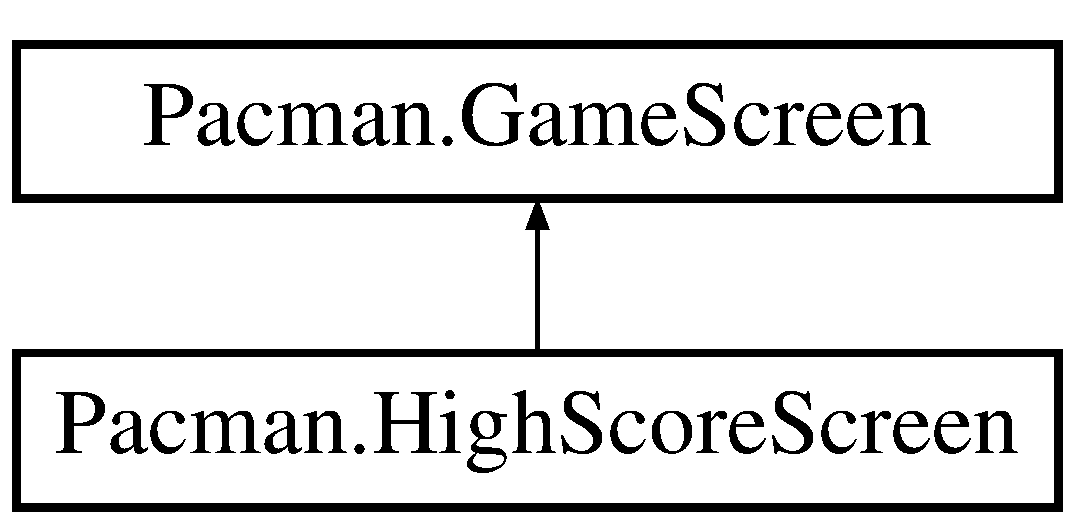
\includegraphics[height=2.000000cm]{class_pacman_1_1_high_score_screen}
\end{center}
\end{figure}
\subsection*{Public Member Functions}
\begin{DoxyCompactItemize}
\item 
override void \hyperlink{class_pacman_1_1_high_score_screen_a2f9c7bd488af9db87c5e74c5e4d21a4e}{Load\-Content} (Content\-Manager Content)
\begin{DoxyCompactList}\small\item\em Initializes the variables and loads the text to be fade-\/animated, loads the highscore from the highscore X\-M\-L file \end{DoxyCompactList}\item 
override void \hyperlink{class_pacman_1_1_high_score_screen_a9486bf7d1079734d5cf842b53c8f4ade}{Unload\-Content} ()
\begin{DoxyCompactList}\small\item\em Unloads the highscore class and fadeanimation class, called when a new screen is added \end{DoxyCompactList}\item 
override void \hyperlink{class_pacman_1_1_high_score_screen_a049329dc007241790cdf1603b0ef69d6}{Update} (Game\-Time game\-Time)
\begin{DoxyCompactList}\small\item\em checks to see if the user has pressed the Enter key, if so change the screen to a Main menu screen \end{DoxyCompactList}\item 
override void \hyperlink{class_pacman_1_1_high_score_screen_ad785f3290cea4ce2483d89dd651bee76}{Draw} (Sprite\-Batch sprite\-Batch)
\begin{DoxyCompactList}\small\item\em Draws the highscore list and text fade animation \end{DoxyCompactList}\end{DoxyCompactItemize}
\subsection*{Additional Inherited Members}


\subsection{Detailed Description}
A screen class that displays the highscore list 



\subsection{Member Function Documentation}
\hypertarget{class_pacman_1_1_high_score_screen_ad785f3290cea4ce2483d89dd651bee76}{\index{Pacman\-::\-High\-Score\-Screen@{Pacman\-::\-High\-Score\-Screen}!Draw@{Draw}}
\index{Draw@{Draw}!Pacman::HighScoreScreen@{Pacman\-::\-High\-Score\-Screen}}
\subsubsection[{Draw}]{\setlength{\rightskip}{0pt plus 5cm}override void Pacman.\-High\-Score\-Screen.\-Draw (
\begin{DoxyParamCaption}
\item[{Sprite\-Batch}]{sprite\-Batch}
\end{DoxyParamCaption}
)\hspace{0.3cm}{\ttfamily [virtual]}}}\label{class_pacman_1_1_high_score_screen_ad785f3290cea4ce2483d89dd651bee76}


Draws the highscore list and text fade animation 


\begin{DoxyParams}{Parameters}
{\em sprite\-Batch} & \\
\hline
\end{DoxyParams}


Reimplemented from \hyperlink{class_pacman_1_1_game_screen_ab7d62816f246e29e70d352d094c36b04}{Pacman.\-Game\-Screen}.

\hypertarget{class_pacman_1_1_high_score_screen_a2f9c7bd488af9db87c5e74c5e4d21a4e}{\index{Pacman\-::\-High\-Score\-Screen@{Pacman\-::\-High\-Score\-Screen}!Load\-Content@{Load\-Content}}
\index{Load\-Content@{Load\-Content}!Pacman::HighScoreScreen@{Pacman\-::\-High\-Score\-Screen}}
\subsubsection[{Load\-Content}]{\setlength{\rightskip}{0pt plus 5cm}override void Pacman.\-High\-Score\-Screen.\-Load\-Content (
\begin{DoxyParamCaption}
\item[{Content\-Manager}]{Content}
\end{DoxyParamCaption}
)\hspace{0.3cm}{\ttfamily [virtual]}}}\label{class_pacman_1_1_high_score_screen_a2f9c7bd488af9db87c5e74c5e4d21a4e}


Initializes the variables and loads the text to be fade-\/animated, loads the highscore from the highscore X\-M\-L file 


\begin{DoxyParams}{Parameters}
{\em Content} & \\
\hline
\end{DoxyParams}


Reimplemented from \hyperlink{class_pacman_1_1_game_screen_a33dbdc943439ae7728aff62b5152aa53}{Pacman.\-Game\-Screen}.

\hypertarget{class_pacman_1_1_high_score_screen_a9486bf7d1079734d5cf842b53c8f4ade}{\index{Pacman\-::\-High\-Score\-Screen@{Pacman\-::\-High\-Score\-Screen}!Unload\-Content@{Unload\-Content}}
\index{Unload\-Content@{Unload\-Content}!Pacman::HighScoreScreen@{Pacman\-::\-High\-Score\-Screen}}
\subsubsection[{Unload\-Content}]{\setlength{\rightskip}{0pt plus 5cm}override void Pacman.\-High\-Score\-Screen.\-Unload\-Content (
\begin{DoxyParamCaption}
{}
\end{DoxyParamCaption}
)\hspace{0.3cm}{\ttfamily [virtual]}}}\label{class_pacman_1_1_high_score_screen_a9486bf7d1079734d5cf842b53c8f4ade}


Unloads the highscore class and fadeanimation class, called when a new screen is added 



Reimplemented from \hyperlink{class_pacman_1_1_game_screen_aa33ba4650a38762eca4bd059fb803942}{Pacman.\-Game\-Screen}.

\hypertarget{class_pacman_1_1_high_score_screen_a049329dc007241790cdf1603b0ef69d6}{\index{Pacman\-::\-High\-Score\-Screen@{Pacman\-::\-High\-Score\-Screen}!Update@{Update}}
\index{Update@{Update}!Pacman::HighScoreScreen@{Pacman\-::\-High\-Score\-Screen}}
\subsubsection[{Update}]{\setlength{\rightskip}{0pt plus 5cm}override void Pacman.\-High\-Score\-Screen.\-Update (
\begin{DoxyParamCaption}
\item[{Game\-Time}]{game\-Time}
\end{DoxyParamCaption}
)\hspace{0.3cm}{\ttfamily [virtual]}}}\label{class_pacman_1_1_high_score_screen_a049329dc007241790cdf1603b0ef69d6}


checks to see if the user has pressed the Enter key, if so change the screen to a Main menu screen 


\begin{DoxyParams}{Parameters}
{\em game\-Time} & \\
\hline
\end{DoxyParams}


Reimplemented from \hyperlink{class_pacman_1_1_game_screen_a768b26cbc3ed823d0dcba5055ae9a8b4}{Pacman.\-Game\-Screen}.



The documentation for this class was generated from the following file\-:\begin{DoxyCompactItemize}
\item 
High\-Score\-Screen.\-cs\end{DoxyCompactItemize}

\hypertarget{class_pacman_1_1_layers}{\section{Pacman.\-Layers Class Reference}
\label{class_pacman_1_1_layers}\index{Pacman.\-Layers@{Pacman.\-Layers}}
}


A dynamic tilemap reader  


\subsection*{Public Member Functions}
\begin{DoxyCompactItemize}
\item 
void \hyperlink{class_pacman_1_1_layers_ae2f8d76ad9fe571a7e0ead57165b402e}{Load\-Content} (Content\-Manager content, string map\-I\-D)
\begin{DoxyCompactList}\small\item\em Loads the tile map from the tilemap text file, adds the single tiles to a layer in which then is added to the tile map. This adds the abillity to read in multiple maps into a single variable. \end{DoxyCompactList}\item 
void \hyperlink{class_pacman_1_1_layers_a721d7d396fb04ab363d485d8474f51a2}{Unload\-Content} ()
\begin{DoxyCompactList}\small\item\em Clears the lists, called when a new screen has been added \end{DoxyCompactList}\item 
void \hyperlink{class_pacman_1_1_layers_a3b799c4834f790a0de8dfdbec02d4974}{Draw} (Sprite\-Batch sprite\-Batch)
\begin{DoxyCompactList}\small\item\em Draws out the map tiles to the screen \end{DoxyCompactList}\end{DoxyCompactItemize}
\subsection*{Properties}
\begin{DoxyCompactItemize}
\item 
\hypertarget{class_pacman_1_1_layers_ad6033d11075ecc2fb07f2366b430c507}{int {\bfseries Layer\-Number}\hspace{0.3cm}{\ttfamily  \mbox{[}set\mbox{]}}}\label{class_pacman_1_1_layers_ad6033d11075ecc2fb07f2366b430c507}

\item 
\hypertarget{class_pacman_1_1_layers_a91d226bdcd4fbde5658b523d547ada8e}{Vector2 {\bfseries Tile\-Dimensions}\hspace{0.3cm}{\ttfamily  \mbox{[}get\mbox{]}}}\label{class_pacman_1_1_layers_a91d226bdcd4fbde5658b523d547ada8e}

\item 
\hypertarget{class_pacman_1_1_layers_af5e3f6ed7cb7ea5a26b5d96930fffb8d}{List$<$ List$<$ List$<$ Vector2 $>$ $>$ $>$ {\bfseries Tile\-Map}\hspace{0.3cm}{\ttfamily  \mbox{[}get, set\mbox{]}}}\label{class_pacman_1_1_layers_af5e3f6ed7cb7ea5a26b5d96930fffb8d}

\end{DoxyCompactItemize}


\subsection{Detailed Description}
A dynamic tilemap reader 



\subsection{Member Function Documentation}
\hypertarget{class_pacman_1_1_layers_a3b799c4834f790a0de8dfdbec02d4974}{\index{Pacman\-::\-Layers@{Pacman\-::\-Layers}!Draw@{Draw}}
\index{Draw@{Draw}!Pacman::Layers@{Pacman\-::\-Layers}}
\subsubsection[{Draw}]{\setlength{\rightskip}{0pt plus 5cm}void Pacman.\-Layers.\-Draw (
\begin{DoxyParamCaption}
\item[{Sprite\-Batch}]{sprite\-Batch}
\end{DoxyParamCaption}
)}}\label{class_pacman_1_1_layers_a3b799c4834f790a0de8dfdbec02d4974}


Draws out the map tiles to the screen 


\begin{DoxyParams}{Parameters}
{\em sprite\-Batch} & \\
\hline
\end{DoxyParams}
\hypertarget{class_pacman_1_1_layers_ae2f8d76ad9fe571a7e0ead57165b402e}{\index{Pacman\-::\-Layers@{Pacman\-::\-Layers}!Load\-Content@{Load\-Content}}
\index{Load\-Content@{Load\-Content}!Pacman::Layers@{Pacman\-::\-Layers}}
\subsubsection[{Load\-Content}]{\setlength{\rightskip}{0pt plus 5cm}void Pacman.\-Layers.\-Load\-Content (
\begin{DoxyParamCaption}
\item[{Content\-Manager}]{content, }
\item[{string}]{map\-I\-D}
\end{DoxyParamCaption}
)}}\label{class_pacman_1_1_layers_ae2f8d76ad9fe571a7e0ead57165b402e}


Loads the tile map from the tilemap text file, adds the single tiles to a layer in which then is added to the tile map. This adds the abillity to read in multiple maps into a single variable. 


\begin{DoxyParams}{Parameters}
{\em content} & \\
\hline
{\em map\-I\-D} & \\
\hline
\end{DoxyParams}
\hypertarget{class_pacman_1_1_layers_a721d7d396fb04ab363d485d8474f51a2}{\index{Pacman\-::\-Layers@{Pacman\-::\-Layers}!Unload\-Content@{Unload\-Content}}
\index{Unload\-Content@{Unload\-Content}!Pacman::Layers@{Pacman\-::\-Layers}}
\subsubsection[{Unload\-Content}]{\setlength{\rightskip}{0pt plus 5cm}void Pacman.\-Layers.\-Unload\-Content (
\begin{DoxyParamCaption}
{}
\end{DoxyParamCaption}
)}}\label{class_pacman_1_1_layers_a721d7d396fb04ab363d485d8474f51a2}


Clears the lists, called when a new screen has been added 



The documentation for this class was generated from the following file\-:\begin{DoxyCompactItemize}
\item 
Layers.\-cs\end{DoxyCompactItemize}

\hypertarget{class_pacman_1_1_main_game}{\section{Pacman.\-Main\-Game Class Reference}
\label{class_pacman_1_1_main_game}\index{Pacman.\-Main\-Game@{Pacman.\-Main\-Game}}
}


The main game screen  


Inheritance diagram for Pacman.\-Main\-Game\-:\begin{figure}[H]
\begin{center}
\leavevmode
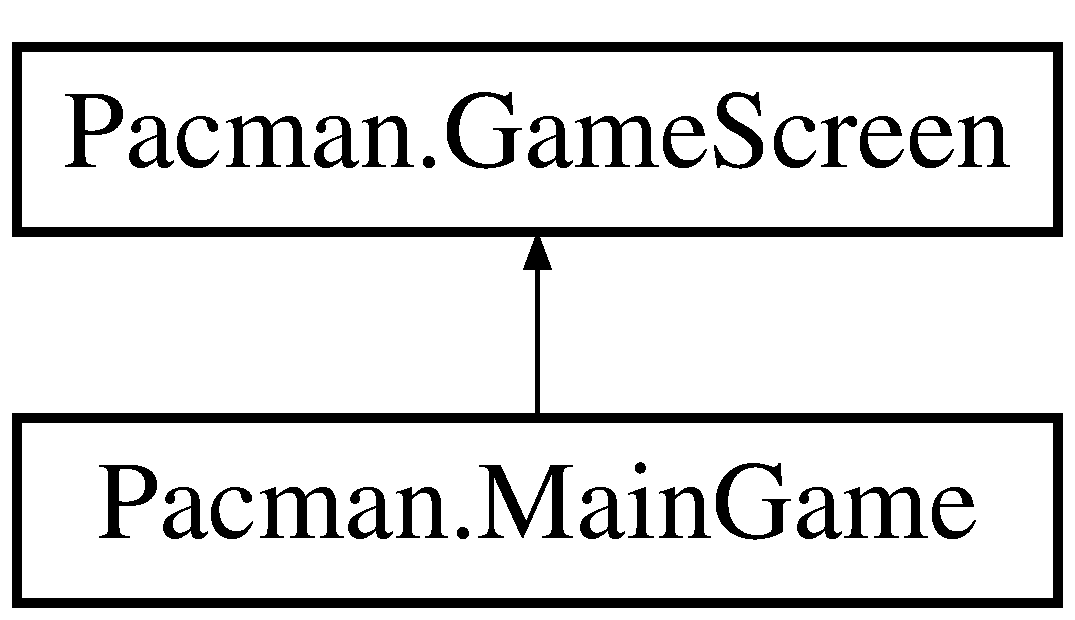
\includegraphics[height=2.000000cm]{class_pacman_1_1_main_game}
\end{center}
\end{figure}
\subsection*{Public Member Functions}
\begin{DoxyCompactItemize}
\item 
override void \hyperlink{class_pacman_1_1_main_game_a8d51b2ec6cc93f142309ea6fe36b2b30}{Load\-Content} (Content\-Manager Content)
\begin{DoxyCompactList}\small\item\em Loads and initializes all the variables, adds three enemies with different \char`\"{}smart levels\char`\"{} \end{DoxyCompactList}\item 
override void \hyperlink{class_pacman_1_1_main_game_abb1d5e7608fa0d9752c0c434cb103e6b}{Update} (Game\-Time game\-Time)
\begin{DoxyCompactList}\small\item\em Updates the enemy and player, checks if the gameover criteria is met, if it is then add the score to the highscore and transition to the gameover screen \end{DoxyCompactList}\item 
override void \hyperlink{class_pacman_1_1_main_game_a7858b061a1db731df54381e03f71b7e0}{Unload\-Content} ()
\begin{DoxyCompactList}\small\item\em Unloads everything, called when a new screen is added \end{DoxyCompactList}\item 
override void \hyperlink{class_pacman_1_1_main_game_ae0723e8c7fcc6fe57383774b84bc5c91}{Draw} (Sprite\-Batch sprite\-Batch)
\begin{DoxyCompactList}\small\item\em Calls the draw function of the map,in-\/game highscore,enemies and player \end{DoxyCompactList}\end{DoxyCompactItemize}
\subsection*{Additional Inherited Members}


\subsection{Detailed Description}
The main game screen 



\subsection{Member Function Documentation}
\hypertarget{class_pacman_1_1_main_game_ae0723e8c7fcc6fe57383774b84bc5c91}{\index{Pacman\-::\-Main\-Game@{Pacman\-::\-Main\-Game}!Draw@{Draw}}
\index{Draw@{Draw}!Pacman::MainGame@{Pacman\-::\-Main\-Game}}
\subsubsection[{Draw}]{\setlength{\rightskip}{0pt plus 5cm}override void Pacman.\-Main\-Game.\-Draw (
\begin{DoxyParamCaption}
\item[{Sprite\-Batch}]{sprite\-Batch}
\end{DoxyParamCaption}
)\hspace{0.3cm}{\ttfamily [virtual]}}}\label{class_pacman_1_1_main_game_ae0723e8c7fcc6fe57383774b84bc5c91}


Calls the draw function of the map,in-\/game highscore,enemies and player 


\begin{DoxyParams}{Parameters}
{\em sprite\-Batch} & \\
\hline
\end{DoxyParams}


Reimplemented from \hyperlink{class_pacman_1_1_game_screen_ab7d62816f246e29e70d352d094c36b04}{Pacman.\-Game\-Screen}.

\hypertarget{class_pacman_1_1_main_game_a8d51b2ec6cc93f142309ea6fe36b2b30}{\index{Pacman\-::\-Main\-Game@{Pacman\-::\-Main\-Game}!Load\-Content@{Load\-Content}}
\index{Load\-Content@{Load\-Content}!Pacman::MainGame@{Pacman\-::\-Main\-Game}}
\subsubsection[{Load\-Content}]{\setlength{\rightskip}{0pt plus 5cm}override void Pacman.\-Main\-Game.\-Load\-Content (
\begin{DoxyParamCaption}
\item[{Content\-Manager}]{Content}
\end{DoxyParamCaption}
)\hspace{0.3cm}{\ttfamily [virtual]}}}\label{class_pacman_1_1_main_game_a8d51b2ec6cc93f142309ea6fe36b2b30}


Loads and initializes all the variables, adds three enemies with different \char`\"{}smart levels\char`\"{} 


\begin{DoxyParams}{Parameters}
{\em Content} & \\
\hline
\end{DoxyParams}


Reimplemented from \hyperlink{class_pacman_1_1_game_screen_a33dbdc943439ae7728aff62b5152aa53}{Pacman.\-Game\-Screen}.

\hypertarget{class_pacman_1_1_main_game_a7858b061a1db731df54381e03f71b7e0}{\index{Pacman\-::\-Main\-Game@{Pacman\-::\-Main\-Game}!Unload\-Content@{Unload\-Content}}
\index{Unload\-Content@{Unload\-Content}!Pacman::MainGame@{Pacman\-::\-Main\-Game}}
\subsubsection[{Unload\-Content}]{\setlength{\rightskip}{0pt plus 5cm}override void Pacman.\-Main\-Game.\-Unload\-Content (
\begin{DoxyParamCaption}
{}
\end{DoxyParamCaption}
)\hspace{0.3cm}{\ttfamily [virtual]}}}\label{class_pacman_1_1_main_game_a7858b061a1db731df54381e03f71b7e0}


Unloads everything, called when a new screen is added 



Reimplemented from \hyperlink{class_pacman_1_1_game_screen_aa33ba4650a38762eca4bd059fb803942}{Pacman.\-Game\-Screen}.

\hypertarget{class_pacman_1_1_main_game_abb1d5e7608fa0d9752c0c434cb103e6b}{\index{Pacman\-::\-Main\-Game@{Pacman\-::\-Main\-Game}!Update@{Update}}
\index{Update@{Update}!Pacman::MainGame@{Pacman\-::\-Main\-Game}}
\subsubsection[{Update}]{\setlength{\rightskip}{0pt plus 5cm}override void Pacman.\-Main\-Game.\-Update (
\begin{DoxyParamCaption}
\item[{Game\-Time}]{game\-Time}
\end{DoxyParamCaption}
)\hspace{0.3cm}{\ttfamily [virtual]}}}\label{class_pacman_1_1_main_game_abb1d5e7608fa0d9752c0c434cb103e6b}


Updates the enemy and player, checks if the gameover criteria is met, if it is then add the score to the highscore and transition to the gameover screen 


\begin{DoxyParams}{Parameters}
{\em game\-Time} & \\
\hline
\end{DoxyParams}


Reimplemented from \hyperlink{class_pacman_1_1_game_screen_a768b26cbc3ed823d0dcba5055ae9a8b4}{Pacman.\-Game\-Screen}.



The documentation for this class was generated from the following file\-:\begin{DoxyCompactItemize}
\item 
Main\-Game.\-cs\end{DoxyCompactItemize}

\hypertarget{class_pacman_1_1_main_menu}{\section{Pacman.\-Main\-Menu Class Reference}
\label{class_pacman_1_1_main_menu}\index{Pacman.\-Main\-Menu@{Pacman.\-Main\-Menu}}
}


The main menu screen, uses the \hyperlink{class_pacman_1_1_menu_manager}{Menu\-Manager} class  


Inheritance diagram for Pacman.\-Main\-Menu\-:\begin{figure}[H]
\begin{center}
\leavevmode
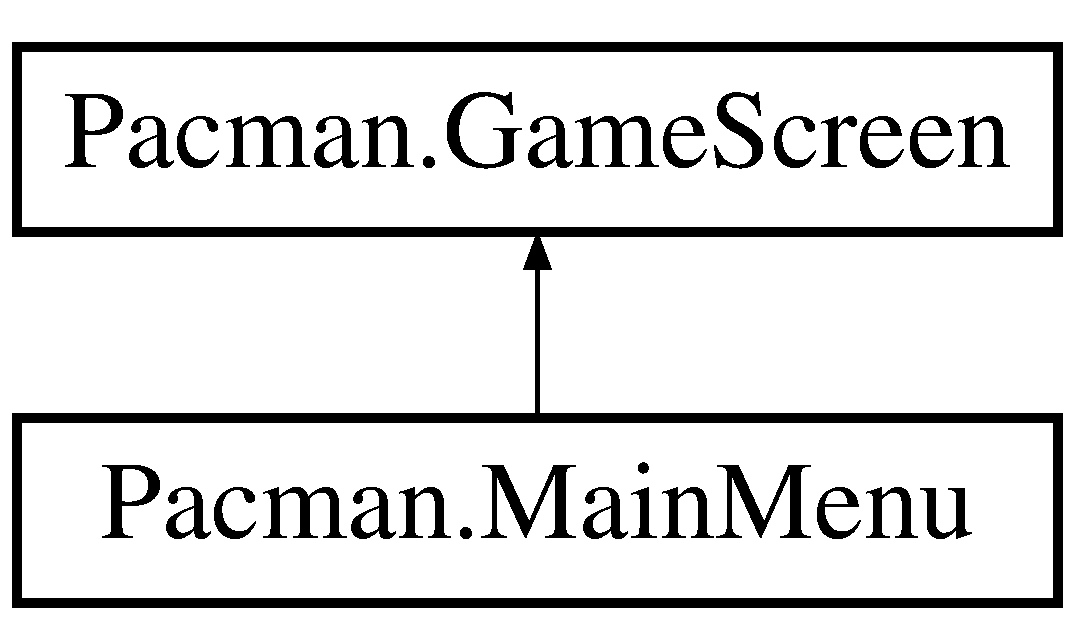
\includegraphics[height=2.000000cm]{class_pacman_1_1_main_menu}
\end{center}
\end{figure}
\subsection*{Public Member Functions}
\begin{DoxyCompactItemize}
\item 
override void \hyperlink{class_pacman_1_1_main_menu_afe334b467dd04341970f6a37521afbd5}{Load\-Content} (Content\-Manager Content)
\begin{DoxyCompactList}\small\item\em Loads the content to the menu class. \end{DoxyCompactList}\item 
override void \hyperlink{class_pacman_1_1_main_menu_a5081e962db4976366a69d7e762680edd}{Unload\-Content} ()
\begin{DoxyCompactList}\small\item\em Unloads the content, called when a new screen has been added \end{DoxyCompactList}\item 
override void \hyperlink{class_pacman_1_1_main_menu_aa93dfb885cc86654e2596168690e44c4}{Update} (Game\-Time game\-Time)
\begin{DoxyCompactList}\small\item\em Updates the menu \end{DoxyCompactList}\item 
override void \hyperlink{class_pacman_1_1_main_menu_aa1ea98563a955497e06808b440a65712}{Draw} (Sprite\-Batch sprite\-Batch)
\begin{DoxyCompactList}\small\item\em Draws the menu \end{DoxyCompactList}\end{DoxyCompactItemize}
\subsection*{Additional Inherited Members}


\subsection{Detailed Description}
The main menu screen, uses the \hyperlink{class_pacman_1_1_menu_manager}{Menu\-Manager} class 



\subsection{Member Function Documentation}
\hypertarget{class_pacman_1_1_main_menu_aa1ea98563a955497e06808b440a65712}{\index{Pacman\-::\-Main\-Menu@{Pacman\-::\-Main\-Menu}!Draw@{Draw}}
\index{Draw@{Draw}!Pacman::MainMenu@{Pacman\-::\-Main\-Menu}}
\subsubsection[{Draw}]{\setlength{\rightskip}{0pt plus 5cm}override void Pacman.\-Main\-Menu.\-Draw (
\begin{DoxyParamCaption}
\item[{Sprite\-Batch}]{sprite\-Batch}
\end{DoxyParamCaption}
)\hspace{0.3cm}{\ttfamily [virtual]}}}\label{class_pacman_1_1_main_menu_aa1ea98563a955497e06808b440a65712}


Draws the menu 


\begin{DoxyParams}{Parameters}
{\em sprite\-Batch} & \\
\hline
\end{DoxyParams}


Reimplemented from \hyperlink{class_pacman_1_1_game_screen_ab7d62816f246e29e70d352d094c36b04}{Pacman.\-Game\-Screen}.

\hypertarget{class_pacman_1_1_main_menu_afe334b467dd04341970f6a37521afbd5}{\index{Pacman\-::\-Main\-Menu@{Pacman\-::\-Main\-Menu}!Load\-Content@{Load\-Content}}
\index{Load\-Content@{Load\-Content}!Pacman::MainMenu@{Pacman\-::\-Main\-Menu}}
\subsubsection[{Load\-Content}]{\setlength{\rightskip}{0pt plus 5cm}override void Pacman.\-Main\-Menu.\-Load\-Content (
\begin{DoxyParamCaption}
\item[{Content\-Manager}]{Content}
\end{DoxyParamCaption}
)\hspace{0.3cm}{\ttfamily [virtual]}}}\label{class_pacman_1_1_main_menu_afe334b467dd04341970f6a37521afbd5}


Loads the content to the menu class. 


\begin{DoxyParams}{Parameters}
{\em Content} & \\
\hline
\end{DoxyParams}


Reimplemented from \hyperlink{class_pacman_1_1_game_screen_a33dbdc943439ae7728aff62b5152aa53}{Pacman.\-Game\-Screen}.

\hypertarget{class_pacman_1_1_main_menu_a5081e962db4976366a69d7e762680edd}{\index{Pacman\-::\-Main\-Menu@{Pacman\-::\-Main\-Menu}!Unload\-Content@{Unload\-Content}}
\index{Unload\-Content@{Unload\-Content}!Pacman::MainMenu@{Pacman\-::\-Main\-Menu}}
\subsubsection[{Unload\-Content}]{\setlength{\rightskip}{0pt plus 5cm}override void Pacman.\-Main\-Menu.\-Unload\-Content (
\begin{DoxyParamCaption}
{}
\end{DoxyParamCaption}
)\hspace{0.3cm}{\ttfamily [virtual]}}}\label{class_pacman_1_1_main_menu_a5081e962db4976366a69d7e762680edd}


Unloads the content, called when a new screen has been added 



Reimplemented from \hyperlink{class_pacman_1_1_game_screen_aa33ba4650a38762eca4bd059fb803942}{Pacman.\-Game\-Screen}.

\hypertarget{class_pacman_1_1_main_menu_aa93dfb885cc86654e2596168690e44c4}{\index{Pacman\-::\-Main\-Menu@{Pacman\-::\-Main\-Menu}!Update@{Update}}
\index{Update@{Update}!Pacman::MainMenu@{Pacman\-::\-Main\-Menu}}
\subsubsection[{Update}]{\setlength{\rightskip}{0pt plus 5cm}override void Pacman.\-Main\-Menu.\-Update (
\begin{DoxyParamCaption}
\item[{Game\-Time}]{game\-Time}
\end{DoxyParamCaption}
)\hspace{0.3cm}{\ttfamily [virtual]}}}\label{class_pacman_1_1_main_menu_aa93dfb885cc86654e2596168690e44c4}


Updates the menu 


\begin{DoxyParams}{Parameters}
{\em game\-Time} & \\
\hline
\end{DoxyParams}


Reimplemented from \hyperlink{class_pacman_1_1_game_screen_a768b26cbc3ed823d0dcba5055ae9a8b4}{Pacman.\-Game\-Screen}.



The documentation for this class was generated from the following file\-:\begin{DoxyCompactItemize}
\item 
Main\-Menu.\-cs\end{DoxyCompactItemize}

\hypertarget{class_pacman_1_1_menu_manager}{\section{Pacman.\-Menu\-Manager Class Reference}
\label{class_pacman_1_1_menu_manager}\index{Pacman.\-Menu\-Manager@{Pacman.\-Menu\-Manager}}
}


A menu manager that is as dynamic as possible  


\subsection*{Public Member Functions}
\begin{DoxyCompactItemize}
\item 
void \hyperlink{class_pacman_1_1_menu_manager_af7008f3b4b1865fc3550336bcccb2bea}{Load\-Content} (Content\-Manager content, string id)
\begin{DoxyCompactList}\small\item\em initializes and loads in the attributes and contents from the menu text file to the manager. \end{DoxyCompactList}\item 
void \hyperlink{class_pacman_1_1_menu_manager_ab48258dd7d618e8e9dbd50229e5da01e}{Unload\-Content} ()
\begin{DoxyCompactList}\small\item\em Clears all the lists and unloads the current contentmanager, called when a new screen has been added \end{DoxyCompactList}\item 
void \hyperlink{class_pacman_1_1_menu_manager_a72d787f7a1545e1b6af8c70cd70e5e95}{Update} (Game\-Time game\-Time)
\begin{DoxyCompactList}\small\item\em Gets user input for the menu, and Activates a new instance for a new screen depending on what the user wanted. And transitions to that specific screen. \end{DoxyCompactList}\item 
void \hyperlink{class_pacman_1_1_menu_manager_a08d0a81648d1d326553435266a5eb488}{Draw} (Sprite\-Batch sprite\-Batch)
\begin{DoxyCompactList}\small\item\em Draws the screen animations \end{DoxyCompactList}\end{DoxyCompactItemize}


\subsection{Detailed Description}
A menu manager that is as dynamic as possible 



\subsection{Member Function Documentation}
\hypertarget{class_pacman_1_1_menu_manager_a08d0a81648d1d326553435266a5eb488}{\index{Pacman\-::\-Menu\-Manager@{Pacman\-::\-Menu\-Manager}!Draw@{Draw}}
\index{Draw@{Draw}!Pacman::MenuManager@{Pacman\-::\-Menu\-Manager}}
\subsubsection[{Draw}]{\setlength{\rightskip}{0pt plus 5cm}void Pacman.\-Menu\-Manager.\-Draw (
\begin{DoxyParamCaption}
\item[{Sprite\-Batch}]{sprite\-Batch}
\end{DoxyParamCaption}
)}}\label{class_pacman_1_1_menu_manager_a08d0a81648d1d326553435266a5eb488}


Draws the screen animations 


\begin{DoxyParams}{Parameters}
{\em sprite\-Batch} & \\
\hline
\end{DoxyParams}
\hypertarget{class_pacman_1_1_menu_manager_af7008f3b4b1865fc3550336bcccb2bea}{\index{Pacman\-::\-Menu\-Manager@{Pacman\-::\-Menu\-Manager}!Load\-Content@{Load\-Content}}
\index{Load\-Content@{Load\-Content}!Pacman::MenuManager@{Pacman\-::\-Menu\-Manager}}
\subsubsection[{Load\-Content}]{\setlength{\rightskip}{0pt plus 5cm}void Pacman.\-Menu\-Manager.\-Load\-Content (
\begin{DoxyParamCaption}
\item[{Content\-Manager}]{content, }
\item[{string}]{id}
\end{DoxyParamCaption}
)}}\label{class_pacman_1_1_menu_manager_af7008f3b4b1865fc3550336bcccb2bea}


initializes and loads in the attributes and contents from the menu text file to the manager. 


\begin{DoxyParams}{Parameters}
{\em content} & \\
\hline
{\em id} & \\
\hline
\end{DoxyParams}
\hypertarget{class_pacman_1_1_menu_manager_ab48258dd7d618e8e9dbd50229e5da01e}{\index{Pacman\-::\-Menu\-Manager@{Pacman\-::\-Menu\-Manager}!Unload\-Content@{Unload\-Content}}
\index{Unload\-Content@{Unload\-Content}!Pacman::MenuManager@{Pacman\-::\-Menu\-Manager}}
\subsubsection[{Unload\-Content}]{\setlength{\rightskip}{0pt plus 5cm}void Pacman.\-Menu\-Manager.\-Unload\-Content (
\begin{DoxyParamCaption}
{}
\end{DoxyParamCaption}
)}}\label{class_pacman_1_1_menu_manager_ab48258dd7d618e8e9dbd50229e5da01e}


Clears all the lists and unloads the current contentmanager, called when a new screen has been added 

\hypertarget{class_pacman_1_1_menu_manager_a72d787f7a1545e1b6af8c70cd70e5e95}{\index{Pacman\-::\-Menu\-Manager@{Pacman\-::\-Menu\-Manager}!Update@{Update}}
\index{Update@{Update}!Pacman::MenuManager@{Pacman\-::\-Menu\-Manager}}
\subsubsection[{Update}]{\setlength{\rightskip}{0pt plus 5cm}void Pacman.\-Menu\-Manager.\-Update (
\begin{DoxyParamCaption}
\item[{Game\-Time}]{game\-Time}
\end{DoxyParamCaption}
)}}\label{class_pacman_1_1_menu_manager_a72d787f7a1545e1b6af8c70cd70e5e95}


Gets user input for the menu, and Activates a new instance for a new screen depending on what the user wanted. And transitions to that specific screen. 


\begin{DoxyParams}{Parameters}
{\em game\-Time} & \\
\hline
\end{DoxyParams}


The documentation for this class was generated from the following file\-:\begin{DoxyCompactItemize}
\item 
Menu\-Manager.\-cs\end{DoxyCompactItemize}

\hypertarget{struct_pacman_1_1_path_finding_1_1_node}{\section{Pacman.\-Path\-Finding.\-Node Struct Reference}
\label{struct_pacman_1_1_path_finding_1_1_node}\index{Pacman.\-Path\-Finding.\-Node@{Pacman.\-Path\-Finding.\-Node}}
}
\subsection*{Public Member Functions}
\begin{DoxyCompactItemize}
\item 
\hypertarget{struct_pacman_1_1_path_finding_1_1_node_a997f021baab5100b2b7848ea005b5bb8}{void {\bfseries Init} ()}\label{struct_pacman_1_1_path_finding_1_1_node_a997f021baab5100b2b7848ea005b5bb8}

\end{DoxyCompactItemize}
\subsection*{Public Attributes}
\begin{DoxyCompactItemize}
\item 
\hypertarget{struct_pacman_1_1_path_finding_1_1_node_a984787c7a12094c294a009addd283d3c}{Node\-State {\bfseries State}}\label{struct_pacman_1_1_path_finding_1_1_node_a984787c7a12094c294a009addd283d3c}

\item 
\hypertarget{struct_pacman_1_1_path_finding_1_1_node_a7cf4681e38de8676a6b22af9a0b2c2f6}{bool {\bfseries wall}}\label{struct_pacman_1_1_path_finding_1_1_node_a7cf4681e38de8676a6b22af9a0b2c2f6}

\item 
\hypertarget{struct_pacman_1_1_path_finding_1_1_node_a3c12ada96c69a8368a78a196bdabddf1}{\hyperlink{struct_pacman_1_1_path_finding_1_1_position}{Position} {\bfseries Parent}}\label{struct_pacman_1_1_path_finding_1_1_node_a3c12ada96c69a8368a78a196bdabddf1}

\item 
\hypertarget{struct_pacman_1_1_path_finding_1_1_node_a5e8fb44081d6fda396e0939372489c60}{int {\bfseries g\-Value}}\label{struct_pacman_1_1_path_finding_1_1_node_a5e8fb44081d6fda396e0939372489c60}

\item 
\hypertarget{struct_pacman_1_1_path_finding_1_1_node_a12375ab3593ca39fb8229cc17f017aa3}{int {\bfseries h\-Value}}\label{struct_pacman_1_1_path_finding_1_1_node_a12375ab3593ca39fb8229cc17f017aa3}

\end{DoxyCompactItemize}
\subsection*{Properties}
\begin{DoxyCompactItemize}
\item 
\hypertarget{struct_pacman_1_1_path_finding_1_1_node_acea93c5cdc25fea4649cb0051db4f991}{int {\bfseries f\-Value}\hspace{0.3cm}{\ttfamily  \mbox{[}get, set\mbox{]}}}\label{struct_pacman_1_1_path_finding_1_1_node_acea93c5cdc25fea4649cb0051db4f991}

\end{DoxyCompactItemize}


The documentation for this struct was generated from the following file\-:\begin{DoxyCompactItemize}
\item 
Path\-Finding.\-cs\end{DoxyCompactItemize}

\hypertarget{class_pacman_1_1_path_finding}{\section{Pacman.\-Path\-Finding Class Reference}
\label{class_pacman_1_1_path_finding}\index{Pacman.\-Path\-Finding@{Pacman.\-Path\-Finding}}
}


A$\ast$ Pathfinding implemented and variable changes, taken from another source.  


\subsection*{Classes}
\begin{DoxyCompactItemize}
\item 
struct \hyperlink{struct_pacman_1_1_path_finding_1_1_node}{Node}
\item 
struct \hyperlink{struct_pacman_1_1_path_finding_1_1_position}{Position}
\end{DoxyCompactItemize}
\subsection*{Public Types}
\begin{DoxyCompactItemize}
\item 
enum {\bfseries Node\-State} \{ \\*
{\bfseries Not\-Visited} = 0, 
{\bfseries Open} = 1, 
{\bfseries Closed} = 2, 
{\bfseries Start} = 3, 
\\*
{\bfseries Goal} = 4, 
{\bfseries Wall} = 5, 
{\bfseries Path\-To\-Goal\-Node\-Found} = 6
 \}
\item 
enum {\bfseries Direction} \{ \\*
{\bfseries None} = 0, 
{\bfseries South} = 1, 
{\bfseries North} = 4, 
{\bfseries West} = 7, 
\\*
{\bfseries East} = 8
 \}
\end{DoxyCompactItemize}
\subsection*{Public Member Functions}
\begin{DoxyCompactItemize}
\item 
void \hyperlink{class_pacman_1_1_path_finding_ab8d7e426f26863d649aba98fbb6ca3d9}{Init} (\hyperlink{class_pacman_1_1_collision}{Collision} col, Vector2 goal\-Position, Vector2 start\-Position)
\begin{DoxyCompactList}\small\item\em Sets the maps rows and collumns, sets the goal and startposition and which nodes have a wall \end{DoxyCompactList}\item 
void \hyperlink{class_pacman_1_1_path_finding_a9e27351b57793d85d58bb5f9743cd780}{Clear\-Path} (\hyperlink{class_pacman_1_1_collision}{Collision} col, Vector2 goal\-Position, Vector2 start\-Position)
\begin{DoxyCompactList}\small\item\em Clears the path \end{DoxyCompactList}\item 
\hypertarget{class_pacman_1_1_path_finding_ad971d9340e21fa692108e23a30b3cef7}{void {\bfseries Path\-Finder} ()}\label{class_pacman_1_1_path_finding_ad971d9340e21fa692108e23a30b3cef7}

\item 
bool \hyperlink{class_pacman_1_1_path_finding_aff5cef225414a175fc55139a5b908ef4}{Path\-Find\-Step} ()
\begin{DoxyCompactList}\small\item\em Searches the horizontal and vertical directions and see if they are not walls, and checks if the current search node is the goal node \end{DoxyCompactList}\item 
Direction \hyperlink{class_pacman_1_1_path_finding_a8ca9a4cf80b3b7cf7b345d193a540c3a}{Parent\-Direction} (int r, int c)
\begin{DoxyCompactList}\small\item\em The parent direction \end{DoxyCompactList}\item 
bool \hyperlink{class_pacman_1_1_path_finding_a1aa5a9d3a5ac6cf29a71999c67314e0e}{calculate\-Path} ()
\begin{DoxyCompactList}\small\item\em If we found our goal node set the path to it \end{DoxyCompactList}\end{DoxyCompactItemize}
\subsection*{Public Attributes}
\begin{DoxyCompactItemize}
\item 
\hypertarget{class_pacman_1_1_path_finding_a739b0e110465c157c4c802fe9b481069}{\hyperlink{struct_pacman_1_1_path_finding_1_1_node}{Node}\mbox{[},\mbox{]} {\bfseries map}}\label{class_pacman_1_1_path_finding_a739b0e110465c157c4c802fe9b481069}

\item 
\hypertarget{class_pacman_1_1_path_finding_a8c41602ec09efcc2232a27b89c41dadd}{\hyperlink{struct_pacman_1_1_path_finding_1_1_position}{Position} {\bfseries start\-Position}}\label{class_pacman_1_1_path_finding_a8c41602ec09efcc2232a27b89c41dadd}

\item 
\hypertarget{class_pacman_1_1_path_finding_ac9990969ccf1ab74098303aa2c472550}{\hyperlink{struct_pacman_1_1_path_finding_1_1_position}{Position} {\bfseries goal\-Position}}\label{class_pacman_1_1_path_finding_ac9990969ccf1ab74098303aa2c472550}

\end{DoxyCompactItemize}
\subsection*{Properties}
\begin{DoxyCompactItemize}
\item 
\hypertarget{class_pacman_1_1_path_finding_a6bec1388af69849568d16a5050174ca5}{Queue$<$ Vector2 $>$ {\bfseries Path}\hspace{0.3cm}{\ttfamily  \mbox{[}get\mbox{]}}}\label{class_pacman_1_1_path_finding_a6bec1388af69849568d16a5050174ca5}

\end{DoxyCompactItemize}


\subsection{Detailed Description}
A$\ast$ Pathfinding implemented and variable changes, taken from another source. 



\subsection{Member Function Documentation}
\hypertarget{class_pacman_1_1_path_finding_a1aa5a9d3a5ac6cf29a71999c67314e0e}{\index{Pacman\-::\-Path\-Finding@{Pacman\-::\-Path\-Finding}!calculate\-Path@{calculate\-Path}}
\index{calculate\-Path@{calculate\-Path}!Pacman::PathFinding@{Pacman\-::\-Path\-Finding}}
\subsubsection[{calculate\-Path}]{\setlength{\rightskip}{0pt plus 5cm}bool Pacman.\-Path\-Finding.\-calculate\-Path (
\begin{DoxyParamCaption}
{}
\end{DoxyParamCaption}
)}}\label{class_pacman_1_1_path_finding_a1aa5a9d3a5ac6cf29a71999c67314e0e}


If we found our goal node set the path to it 

\begin{DoxyReturn}{Returns}

\end{DoxyReturn}
\hypertarget{class_pacman_1_1_path_finding_a9e27351b57793d85d58bb5f9743cd780}{\index{Pacman\-::\-Path\-Finding@{Pacman\-::\-Path\-Finding}!Clear\-Path@{Clear\-Path}}
\index{Clear\-Path@{Clear\-Path}!Pacman::PathFinding@{Pacman\-::\-Path\-Finding}}
\subsubsection[{Clear\-Path}]{\setlength{\rightskip}{0pt plus 5cm}void Pacman.\-Path\-Finding.\-Clear\-Path (
\begin{DoxyParamCaption}
\item[{{\bf Collision}}]{col, }
\item[{Vector2}]{goal\-Position, }
\item[{Vector2}]{start\-Position}
\end{DoxyParamCaption}
)}}\label{class_pacman_1_1_path_finding_a9e27351b57793d85d58bb5f9743cd780}


Clears the path 


\begin{DoxyParams}{Parameters}
{\em col} & \\
\hline
{\em goal\-Position} & \\
\hline
{\em start\-Position} & \\
\hline
\end{DoxyParams}
\hypertarget{class_pacman_1_1_path_finding_ab8d7e426f26863d649aba98fbb6ca3d9}{\index{Pacman\-::\-Path\-Finding@{Pacman\-::\-Path\-Finding}!Init@{Init}}
\index{Init@{Init}!Pacman::PathFinding@{Pacman\-::\-Path\-Finding}}
\subsubsection[{Init}]{\setlength{\rightskip}{0pt plus 5cm}void Pacman.\-Path\-Finding.\-Init (
\begin{DoxyParamCaption}
\item[{{\bf Collision}}]{col, }
\item[{Vector2}]{goal\-Position, }
\item[{Vector2}]{start\-Position}
\end{DoxyParamCaption}
)}}\label{class_pacman_1_1_path_finding_ab8d7e426f26863d649aba98fbb6ca3d9}


Sets the maps rows and collumns, sets the goal and startposition and which nodes have a wall 


\begin{DoxyParams}{Parameters}
{\em col} & \\
\hline
{\em goal\-Position} & \\
\hline
{\em start\-Position} & \\
\hline
\end{DoxyParams}
\hypertarget{class_pacman_1_1_path_finding_a8ca9a4cf80b3b7cf7b345d193a540c3a}{\index{Pacman\-::\-Path\-Finding@{Pacman\-::\-Path\-Finding}!Parent\-Direction@{Parent\-Direction}}
\index{Parent\-Direction@{Parent\-Direction}!Pacman::PathFinding@{Pacman\-::\-Path\-Finding}}
\subsubsection[{Parent\-Direction}]{\setlength{\rightskip}{0pt plus 5cm}Direction Pacman.\-Path\-Finding.\-Parent\-Direction (
\begin{DoxyParamCaption}
\item[{int}]{r, }
\item[{int}]{c}
\end{DoxyParamCaption}
)}}\label{class_pacman_1_1_path_finding_a8ca9a4cf80b3b7cf7b345d193a540c3a}


The parent direction 


\begin{DoxyParams}{Parameters}
{\em r} & \\
\hline
{\em c} & \\
\hline
\end{DoxyParams}
\begin{DoxyReturn}{Returns}

\end{DoxyReturn}
\hypertarget{class_pacman_1_1_path_finding_aff5cef225414a175fc55139a5b908ef4}{\index{Pacman\-::\-Path\-Finding@{Pacman\-::\-Path\-Finding}!Path\-Find\-Step@{Path\-Find\-Step}}
\index{Path\-Find\-Step@{Path\-Find\-Step}!Pacman::PathFinding@{Pacman\-::\-Path\-Finding}}
\subsubsection[{Path\-Find\-Step}]{\setlength{\rightskip}{0pt plus 5cm}bool Pacman.\-Path\-Finding.\-Path\-Find\-Step (
\begin{DoxyParamCaption}
{}
\end{DoxyParamCaption}
)}}\label{class_pacman_1_1_path_finding_aff5cef225414a175fc55139a5b908ef4}


Searches the horizontal and vertical directions and see if they are not walls, and checks if the current search node is the goal node 

\begin{DoxyReturn}{Returns}

\end{DoxyReturn}


The documentation for this class was generated from the following file\-:\begin{DoxyCompactItemize}
\item 
Path\-Finding.\-cs\end{DoxyCompactItemize}

\hypertarget{class_pacman_1_1_player}{\section{Pacman.\-Player Class Reference}
\label{class_pacman_1_1_player}\index{Pacman.\-Player@{Pacman.\-Player}}
}


The player class  


\subsection*{Public Member Functions}
\begin{DoxyCompactItemize}
\item 
void \hyperlink{class_pacman_1_1_player_aba5e30a8301ffc0ab664300d95ab9743}{Init} ()
\begin{DoxyCompactList}\small\item\em Sets the start position of the player. Sets the amount of frames the player animation have. \end{DoxyCompactList}\item 
void \hyperlink{class_pacman_1_1_player_ab8c4719d16a15c9574a8013807602465}{Load\-Content} (Content\-Manager Content)
\begin{DoxyCompactList}\small\item\em Loads in the animation image and the position of the animation. \end{DoxyCompactList}\item 
void \hyperlink{class_pacman_1_1_player_a68af2a48b6d3f9512ee28aaa30a71f48}{Unload\-Content} ()
\begin{DoxyCompactList}\small\item\em Unloads the variables, called when a new screen has been added \end{DoxyCompactList}\item 
void \hyperlink{class_pacman_1_1_player_af638b60bf7a47f1f31d5ce8b49574d49}{Update} (Game\-Time game\-Time, \hyperlink{class_pacman_1_1_collision}{Collision} col, \hyperlink{class_pacman_1_1_layers}{Layers} layer, \hyperlink{class_pacman_1_1_high_score}{High\-Score} high\-Score)
\begin{DoxyCompactList}\small\item\em Moves the player depending on player input direction, checks collision with walls and food. Increases the highscore by 10 for eatch food eaten. Sets what animation direction that should be drawn. \end{DoxyCompactList}\item 
void \hyperlink{class_pacman_1_1_player_a5b1cc5c97a3a5a1288b8612bd640e9f7}{Draw} (Sprite\-Batch sprite\-Batch)
\begin{DoxyCompactList}\small\item\em Draws the player animation \end{DoxyCompactList}\end{DoxyCompactItemize}
\subsection*{Properties}
\begin{DoxyCompactItemize}
\item 
\hypertarget{class_pacman_1_1_player_a1f0b9092b8260c31d00835b8cec8540f}{Vector2 {\bfseries Player\-Position}\hspace{0.3cm}{\ttfamily  \mbox{[}get\mbox{]}}}\label{class_pacman_1_1_player_a1f0b9092b8260c31d00835b8cec8540f}

\end{DoxyCompactItemize}


\subsection{Detailed Description}
The player class 



\subsection{Member Function Documentation}
\hypertarget{class_pacman_1_1_player_a5b1cc5c97a3a5a1288b8612bd640e9f7}{\index{Pacman\-::\-Player@{Pacman\-::\-Player}!Draw@{Draw}}
\index{Draw@{Draw}!Pacman::Player@{Pacman\-::\-Player}}
\subsubsection[{Draw}]{\setlength{\rightskip}{0pt plus 5cm}void Pacman.\-Player.\-Draw (
\begin{DoxyParamCaption}
\item[{Sprite\-Batch}]{sprite\-Batch}
\end{DoxyParamCaption}
)}}\label{class_pacman_1_1_player_a5b1cc5c97a3a5a1288b8612bd640e9f7}


Draws the player animation 


\begin{DoxyParams}{Parameters}
{\em sprite\-Batch} & \\
\hline
\end{DoxyParams}
\hypertarget{class_pacman_1_1_player_aba5e30a8301ffc0ab664300d95ab9743}{\index{Pacman\-::\-Player@{Pacman\-::\-Player}!Init@{Init}}
\index{Init@{Init}!Pacman::Player@{Pacman\-::\-Player}}
\subsubsection[{Init}]{\setlength{\rightskip}{0pt plus 5cm}void Pacman.\-Player.\-Init (
\begin{DoxyParamCaption}
{}
\end{DoxyParamCaption}
)}}\label{class_pacman_1_1_player_aba5e30a8301ffc0ab664300d95ab9743}


Sets the start position of the player. Sets the amount of frames the player animation have. 

\hypertarget{class_pacman_1_1_player_ab8c4719d16a15c9574a8013807602465}{\index{Pacman\-::\-Player@{Pacman\-::\-Player}!Load\-Content@{Load\-Content}}
\index{Load\-Content@{Load\-Content}!Pacman::Player@{Pacman\-::\-Player}}
\subsubsection[{Load\-Content}]{\setlength{\rightskip}{0pt plus 5cm}void Pacman.\-Player.\-Load\-Content (
\begin{DoxyParamCaption}
\item[{Content\-Manager}]{Content}
\end{DoxyParamCaption}
)}}\label{class_pacman_1_1_player_ab8c4719d16a15c9574a8013807602465}


Loads in the animation image and the position of the animation. 


\begin{DoxyParams}{Parameters}
{\em Content} & \\
\hline
\end{DoxyParams}
\hypertarget{class_pacman_1_1_player_a68af2a48b6d3f9512ee28aaa30a71f48}{\index{Pacman\-::\-Player@{Pacman\-::\-Player}!Unload\-Content@{Unload\-Content}}
\index{Unload\-Content@{Unload\-Content}!Pacman::Player@{Pacman\-::\-Player}}
\subsubsection[{Unload\-Content}]{\setlength{\rightskip}{0pt plus 5cm}void Pacman.\-Player.\-Unload\-Content (
\begin{DoxyParamCaption}
{}
\end{DoxyParamCaption}
)}}\label{class_pacman_1_1_player_a68af2a48b6d3f9512ee28aaa30a71f48}


Unloads the variables, called when a new screen has been added 

\hypertarget{class_pacman_1_1_player_af638b60bf7a47f1f31d5ce8b49574d49}{\index{Pacman\-::\-Player@{Pacman\-::\-Player}!Update@{Update}}
\index{Update@{Update}!Pacman::Player@{Pacman\-::\-Player}}
\subsubsection[{Update}]{\setlength{\rightskip}{0pt plus 5cm}void Pacman.\-Player.\-Update (
\begin{DoxyParamCaption}
\item[{Game\-Time}]{game\-Time, }
\item[{{\bf Collision}}]{col, }
\item[{{\bf Layers}}]{layer, }
\item[{{\bf High\-Score}}]{high\-Score}
\end{DoxyParamCaption}
)}}\label{class_pacman_1_1_player_af638b60bf7a47f1f31d5ce8b49574d49}


Moves the player depending on player input direction, checks collision with walls and food. Increases the highscore by 10 for eatch food eaten. Sets what animation direction that should be drawn. 


\begin{DoxyParams}{Parameters}
{\em game\-Time} & \\
\hline
{\em col} & \\
\hline
{\em layer} & \\
\hline
{\em high\-Score} & \\
\hline
\end{DoxyParams}


The documentation for this class was generated from the following file\-:\begin{DoxyCompactItemize}
\item 
Player.\-cs\end{DoxyCompactItemize}

\hypertarget{struct_pacman_1_1_path_finding_1_1_position}{\section{Pacman.\-Path\-Finding.\-Position Struct Reference}
\label{struct_pacman_1_1_path_finding_1_1_position}\index{Pacman.\-Path\-Finding.\-Position@{Pacman.\-Path\-Finding.\-Position}}
}
\subsection*{Public Member Functions}
\begin{DoxyCompactItemize}
\item 
\hypertarget{struct_pacman_1_1_path_finding_1_1_position_a27ad3ace449adbbf211deebff53c7133}{{\bfseries Position} (int x, int y)}\label{struct_pacman_1_1_path_finding_1_1_position_a27ad3ace449adbbf211deebff53c7133}

\end{DoxyCompactItemize}
\subsection*{Public Attributes}
\begin{DoxyCompactItemize}
\item 
\hypertarget{struct_pacman_1_1_path_finding_1_1_position_a3ba72b69e0c2b9a9e1298f0696f95c27}{int {\bfseries x}}\label{struct_pacman_1_1_path_finding_1_1_position_a3ba72b69e0c2b9a9e1298f0696f95c27}

\item 
\hypertarget{struct_pacman_1_1_path_finding_1_1_position_aede85751ad51b3d8e4a5788332898d7b}{int {\bfseries y}}\label{struct_pacman_1_1_path_finding_1_1_position_aede85751ad51b3d8e4a5788332898d7b}

\end{DoxyCompactItemize}


The documentation for this struct was generated from the following file\-:\begin{DoxyCompactItemize}
\item 
Path\-Finding.\-cs\end{DoxyCompactItemize}

\hypertarget{class_pacman_1_1_screen_animation}{\section{Pacman.\-Screen\-Animation Class Reference}
\label{class_pacman_1_1_screen_animation}\index{Pacman.\-Screen\-Animation@{Pacman.\-Screen\-Animation}}
}


A base class for every screens animation  


Inheritance diagram for Pacman.\-Screen\-Animation\-:\begin{figure}[H]
\begin{center}
\leavevmode
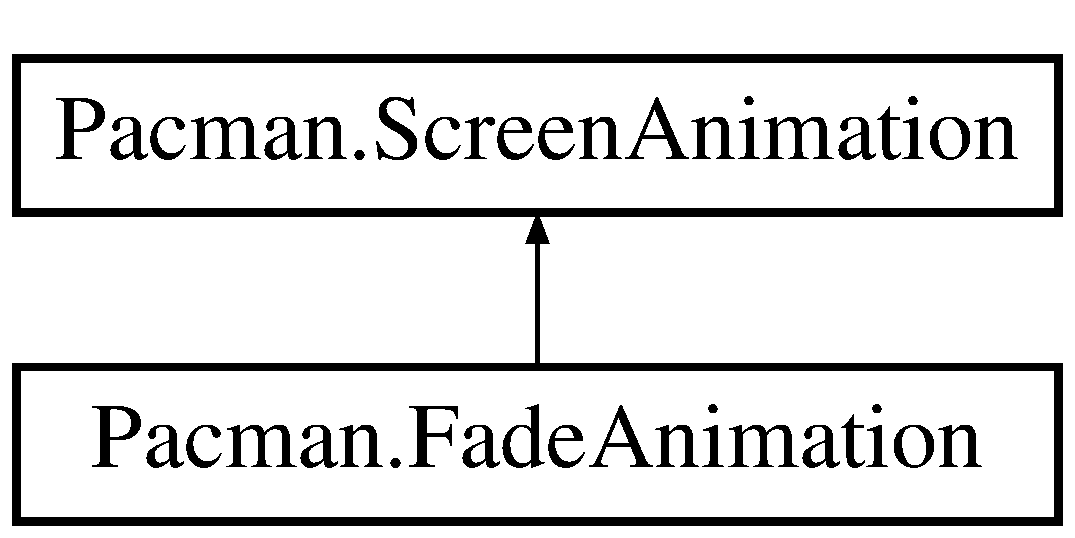
\includegraphics[height=2.000000cm]{class_pacman_1_1_screen_animation}
\end{center}
\end{figure}
\subsection*{Public Member Functions}
\begin{DoxyCompactItemize}
\item 
virtual void \hyperlink{class_pacman_1_1_screen_animation_a566ecb3dca9f82c4eb51f4e3a4019550}{Load\-Content} (Content\-Manager Content, Texture2\-D image, string text, Vector2 position, string font\-I\-D)
\begin{DoxyCompactList}\small\item\em Loads in an image if it's given or a string of text if it is given with the font given \end{DoxyCompactList}\item 
virtual void \hyperlink{class_pacman_1_1_screen_animation_ad9bf49699b6905423cc17047e36e9a1c}{Unload\-Content} ()
\begin{DoxyCompactList}\small\item\em Virtual function that unloads the variables, called when a new screen has been added \end{DoxyCompactList}\item 
virtual void \hyperlink{class_pacman_1_1_screen_animation_af381913622005dfb6b759f7495b37ded}{Update} (Game\-Time game\-Time)
\begin{DoxyCompactList}\small\item\em Virtual update method \end{DoxyCompactList}\item 
void \hyperlink{class_pacman_1_1_screen_animation_aab67af6395aea7e03c7d4d4f6eff9977}{Draw} (Sprite\-Batch sprite\-Batch)
\begin{DoxyCompactList}\small\item\em Draws the string and or image \end{DoxyCompactList}\end{DoxyCompactItemize}
\subsection*{Protected Attributes}
\begin{DoxyCompactItemize}
\item 
\hypertarget{class_pacman_1_1_screen_animation_ac33fed9de162fb2f159f1ad15d3a4d94}{Texture2\-D {\bfseries image}}\label{class_pacman_1_1_screen_animation_ac33fed9de162fb2f159f1ad15d3a4d94}

\item 
\hypertarget{class_pacman_1_1_screen_animation_ab4c0b055eeb0919cf3e30db19d8f15bb}{string {\bfseries text}}\label{class_pacman_1_1_screen_animation_ab4c0b055eeb0919cf3e30db19d8f15bb}

\item 
\hypertarget{class_pacman_1_1_screen_animation_ae014c883301c9f42e00eafcdd513e0d1}{Sprite\-Font {\bfseries font}}\label{class_pacman_1_1_screen_animation_ae014c883301c9f42e00eafcdd513e0d1}

\item 
\hypertarget{class_pacman_1_1_screen_animation_a5a7a6cb6955a0625d6a4ea34fa04166b}{Color {\bfseries color}}\label{class_pacman_1_1_screen_animation_a5a7a6cb6955a0625d6a4ea34fa04166b}

\item 
\hypertarget{class_pacman_1_1_screen_animation_a79065b7a8f285c5f8d67e758ea0f2745}{Rectangle {\bfseries source\-Rect}}\label{class_pacman_1_1_screen_animation_a79065b7a8f285c5f8d67e758ea0f2745}

\item 
\hypertarget{class_pacman_1_1_screen_animation_abef49f89085550929de700f913b22344}{Content\-Manager {\bfseries content}}\label{class_pacman_1_1_screen_animation_abef49f89085550929de700f913b22344}

\item 
\hypertarget{class_pacman_1_1_screen_animation_a9c13f7f141cd083413f2d710aee04b66}{bool {\bfseries active}}\label{class_pacman_1_1_screen_animation_a9c13f7f141cd083413f2d710aee04b66}

\item 
\hypertarget{class_pacman_1_1_screen_animation_a86b87e39731428e90158eabc64a29a60}{float {\bfseries rotation}}\label{class_pacman_1_1_screen_animation_a86b87e39731428e90158eabc64a29a60}

\item 
\hypertarget{class_pacman_1_1_screen_animation_acdac56ee31eec0dc6021ed135b403bf1}{Vector2 {\bfseries origin}}\label{class_pacman_1_1_screen_animation_acdac56ee31eec0dc6021ed135b403bf1}

\item 
\hypertarget{class_pacman_1_1_screen_animation_a33d8bebcfb554857c41a0701e3f05f83}{float {\bfseries alpha}}\label{class_pacman_1_1_screen_animation_a33d8bebcfb554857c41a0701e3f05f83}

\end{DoxyCompactItemize}
\subsection*{Properties}
\begin{DoxyCompactItemize}
\item 
\hypertarget{class_pacman_1_1_screen_animation_a7b643f454b3e1f0faed8959ccd52d4ec}{virtual float {\bfseries Alpha}\hspace{0.3cm}{\ttfamily  \mbox{[}get, set\mbox{]}}}\label{class_pacman_1_1_screen_animation_a7b643f454b3e1f0faed8959ccd52d4ec}

\item 
\hypertarget{class_pacman_1_1_screen_animation_a5d941d20b56fa63c1c289cbcf2b37aec}{bool {\bfseries Active}\hspace{0.3cm}{\ttfamily  \mbox{[}get, set\mbox{]}}}\label{class_pacman_1_1_screen_animation_a5d941d20b56fa63c1c289cbcf2b37aec}

\item 
\hypertarget{class_pacman_1_1_screen_animation_a2a9783313a2891196b9ac1738c00acc4}{float {\bfseries Scale}\hspace{0.3cm}{\ttfamily  \mbox{[}set\mbox{]}}}\label{class_pacman_1_1_screen_animation_a2a9783313a2891196b9ac1738c00acc4}

\end{DoxyCompactItemize}


\subsection{Detailed Description}
A base class for every screens animation 



\subsection{Member Function Documentation}
\hypertarget{class_pacman_1_1_screen_animation_aab67af6395aea7e03c7d4d4f6eff9977}{\index{Pacman\-::\-Screen\-Animation@{Pacman\-::\-Screen\-Animation}!Draw@{Draw}}
\index{Draw@{Draw}!Pacman::ScreenAnimation@{Pacman\-::\-Screen\-Animation}}
\subsubsection[{Draw}]{\setlength{\rightskip}{0pt plus 5cm}void Pacman.\-Screen\-Animation.\-Draw (
\begin{DoxyParamCaption}
\item[{Sprite\-Batch}]{sprite\-Batch}
\end{DoxyParamCaption}
)}}\label{class_pacman_1_1_screen_animation_aab67af6395aea7e03c7d4d4f6eff9977}


Draws the string and or image 


\begin{DoxyParams}{Parameters}
{\em sprite\-Batch} & \\
\hline
\end{DoxyParams}
\hypertarget{class_pacman_1_1_screen_animation_a566ecb3dca9f82c4eb51f4e3a4019550}{\index{Pacman\-::\-Screen\-Animation@{Pacman\-::\-Screen\-Animation}!Load\-Content@{Load\-Content}}
\index{Load\-Content@{Load\-Content}!Pacman::ScreenAnimation@{Pacman\-::\-Screen\-Animation}}
\subsubsection[{Load\-Content}]{\setlength{\rightskip}{0pt plus 5cm}virtual void Pacman.\-Screen\-Animation.\-Load\-Content (
\begin{DoxyParamCaption}
\item[{Content\-Manager}]{Content, }
\item[{Texture2\-D}]{image, }
\item[{string}]{text, }
\item[{Vector2}]{position, }
\item[{string}]{font\-I\-D}
\end{DoxyParamCaption}
)\hspace{0.3cm}{\ttfamily [virtual]}}}\label{class_pacman_1_1_screen_animation_a566ecb3dca9f82c4eb51f4e3a4019550}


Loads in an image if it's given or a string of text if it is given with the font given 


\begin{DoxyParams}{Parameters}
{\em Content} & \\
\hline
{\em image} & \\
\hline
{\em text} & \\
\hline
{\em position} & \\
\hline
{\em font\-I\-D} & \\
\hline
\end{DoxyParams}


Reimplemented in \hyperlink{class_pacman_1_1_fade_animation_a6abddfcfb03a31152da73b6766e99a9d}{Pacman.\-Fade\-Animation}.

\hypertarget{class_pacman_1_1_screen_animation_ad9bf49699b6905423cc17047e36e9a1c}{\index{Pacman\-::\-Screen\-Animation@{Pacman\-::\-Screen\-Animation}!Unload\-Content@{Unload\-Content}}
\index{Unload\-Content@{Unload\-Content}!Pacman::ScreenAnimation@{Pacman\-::\-Screen\-Animation}}
\subsubsection[{Unload\-Content}]{\setlength{\rightskip}{0pt plus 5cm}virtual void Pacman.\-Screen\-Animation.\-Unload\-Content (
\begin{DoxyParamCaption}
{}
\end{DoxyParamCaption}
)\hspace{0.3cm}{\ttfamily [virtual]}}}\label{class_pacman_1_1_screen_animation_ad9bf49699b6905423cc17047e36e9a1c}


Virtual function that unloads the variables, called when a new screen has been added 

\hypertarget{class_pacman_1_1_screen_animation_af381913622005dfb6b759f7495b37ded}{\index{Pacman\-::\-Screen\-Animation@{Pacman\-::\-Screen\-Animation}!Update@{Update}}
\index{Update@{Update}!Pacman::ScreenAnimation@{Pacman\-::\-Screen\-Animation}}
\subsubsection[{Update}]{\setlength{\rightskip}{0pt plus 5cm}virtual void Pacman.\-Screen\-Animation.\-Update (
\begin{DoxyParamCaption}
\item[{Game\-Time}]{game\-Time}
\end{DoxyParamCaption}
)\hspace{0.3cm}{\ttfamily [virtual]}}}\label{class_pacman_1_1_screen_animation_af381913622005dfb6b759f7495b37ded}


Virtual update method 


\begin{DoxyParams}{Parameters}
{\em game\-Time} & \\
\hline
\end{DoxyParams}


Reimplemented in \hyperlink{class_pacman_1_1_fade_animation_ac6d7c4a5845a19f47dd2501271ecee7a}{Pacman.\-Fade\-Animation}.



The documentation for this class was generated from the following file\-:\begin{DoxyCompactItemize}
\item 
Screen\-Animation.\-cs\end{DoxyCompactItemize}

\hypertarget{class_pacman_1_1_screen_manager}{\section{Pacman.\-Screen\-Manager Class Reference}
\label{class_pacman_1_1_screen_manager}\index{Pacman.\-Screen\-Manager@{Pacman.\-Screen\-Manager}}
}


Screen manager that takes care of loading,unloading,updating and drawing of all the screens  


\subsection*{Public Member Functions}
\begin{DoxyCompactItemize}
\item 
void \hyperlink{class_pacman_1_1_screen_manager_a310cc24307ddb1a45dd88e3abc6eafbf}{Add\-Screen} (\hyperlink{class_pacman_1_1_game_screen}{Game\-Screen} screen)
\begin{DoxyCompactList}\small\item\em Sets transision to a new screen. Adds a screen to new\-Screen \end{DoxyCompactList}\item 
void \hyperlink{class_pacman_1_1_screen_manager_ae53ab14c72d98db3b0a92775a24d0cb0}{Add\-Screen} (\hyperlink{class_pacman_1_1_game_screen}{Game\-Screen} screen, float alpha)
\begin{DoxyCompactList}\small\item\em Overloaded version, changes the alpha so it will fade back instead of just switching a screen back instantly, usable when you want a smooth transition between screens. \end{DoxyCompactList}\item 
void \hyperlink{class_pacman_1_1_screen_manager_ababbf590c315370355a1c76e57e61552}{Init} ()
\begin{DoxyCompactList}\small\item\em When the game starts the splash screen will show and a new fade animation will be initialized \end{DoxyCompactList}\item 
void \hyperlink{class_pacman_1_1_screen_manager_ad20ca7f52ff926b637c26d19865f585c}{Load\-Content} (Content\-Manager Content)
\begin{DoxyCompactList}\small\item\em Loads in the contentmanager and fade transistion animation. Calls the loadcontent function of the current screen. \end{DoxyCompactList}\item 
bool \hyperlink{class_pacman_1_1_screen_manager_a1ec7dc1ef0d31e3d8db362644ae0351b}{Update} (Game\-Time game\-Time)
\begin{DoxyCompactList}\small\item\em calls the update function of the current screen, check and return the value from the exit function of the current screen. \end{DoxyCompactList}\item 
void \hyperlink{class_pacman_1_1_screen_manager_ae9477d036da420ac6754c75603f38d08}{Unload\-Content} ()
\begin{DoxyCompactList}\small\item\em Calls the unloadcontent functions for the current screen and clears the screen stack, unloads the fade animation. \end{DoxyCompactList}\item 
void \hyperlink{class_pacman_1_1_screen_manager_ae5011a30dc8765de4dd061cba48c7f89}{Draw} (Sprite\-Batch sprite\-Batch)
\begin{DoxyCompactList}\small\item\em Calls the drawfunction of the current screen. and calls the draw function if we are transitioning between screens \end{DoxyCompactList}\end{DoxyCompactItemize}
\subsection*{Properties}
\begin{DoxyCompactItemize}
\item 
\hypertarget{class_pacman_1_1_screen_manager_a6632eccad8f05e37af385c0c2b230250}{static \hyperlink{class_pacman_1_1_screen_manager}{Screen\-Manager} {\bfseries Instance}\hspace{0.3cm}{\ttfamily  \mbox{[}get\mbox{]}}}\label{class_pacman_1_1_screen_manager_a6632eccad8f05e37af385c0c2b230250}

\item 
\hypertarget{class_pacman_1_1_screen_manager_aa830efd676bbf0af192ac4a0c70b9dfb}{Vector2 {\bfseries Dimensions}\hspace{0.3cm}{\ttfamily  \mbox{[}get, set\mbox{]}}}\label{class_pacman_1_1_screen_manager_aa830efd676bbf0af192ac4a0c70b9dfb}

\end{DoxyCompactItemize}


\subsection{Detailed Description}
Screen manager that takes care of loading,unloading,updating and drawing of all the screens 



\subsection{Member Function Documentation}
\hypertarget{class_pacman_1_1_screen_manager_a310cc24307ddb1a45dd88e3abc6eafbf}{\index{Pacman\-::\-Screen\-Manager@{Pacman\-::\-Screen\-Manager}!Add\-Screen@{Add\-Screen}}
\index{Add\-Screen@{Add\-Screen}!Pacman::ScreenManager@{Pacman\-::\-Screen\-Manager}}
\subsubsection[{Add\-Screen}]{\setlength{\rightskip}{0pt plus 5cm}void Pacman.\-Screen\-Manager.\-Add\-Screen (
\begin{DoxyParamCaption}
\item[{{\bf Game\-Screen}}]{screen}
\end{DoxyParamCaption}
)}}\label{class_pacman_1_1_screen_manager_a310cc24307ddb1a45dd88e3abc6eafbf}


Sets transision to a new screen. Adds a screen to new\-Screen 


\begin{DoxyParams}{Parameters}
{\em screen} & \\
\hline
\end{DoxyParams}
\hypertarget{class_pacman_1_1_screen_manager_ae53ab14c72d98db3b0a92775a24d0cb0}{\index{Pacman\-::\-Screen\-Manager@{Pacman\-::\-Screen\-Manager}!Add\-Screen@{Add\-Screen}}
\index{Add\-Screen@{Add\-Screen}!Pacman::ScreenManager@{Pacman\-::\-Screen\-Manager}}
\subsubsection[{Add\-Screen}]{\setlength{\rightskip}{0pt plus 5cm}void Pacman.\-Screen\-Manager.\-Add\-Screen (
\begin{DoxyParamCaption}
\item[{{\bf Game\-Screen}}]{screen, }
\item[{float}]{alpha}
\end{DoxyParamCaption}
)}}\label{class_pacman_1_1_screen_manager_ae53ab14c72d98db3b0a92775a24d0cb0}


Overloaded version, changes the alpha so it will fade back instead of just switching a screen back instantly, usable when you want a smooth transition between screens. 


\begin{DoxyParams}{Parameters}
{\em screen} & \\
\hline
{\em alpha} & \\
\hline
\end{DoxyParams}
\hypertarget{class_pacman_1_1_screen_manager_ae5011a30dc8765de4dd061cba48c7f89}{\index{Pacman\-::\-Screen\-Manager@{Pacman\-::\-Screen\-Manager}!Draw@{Draw}}
\index{Draw@{Draw}!Pacman::ScreenManager@{Pacman\-::\-Screen\-Manager}}
\subsubsection[{Draw}]{\setlength{\rightskip}{0pt plus 5cm}void Pacman.\-Screen\-Manager.\-Draw (
\begin{DoxyParamCaption}
\item[{Sprite\-Batch}]{sprite\-Batch}
\end{DoxyParamCaption}
)}}\label{class_pacman_1_1_screen_manager_ae5011a30dc8765de4dd061cba48c7f89}


Calls the drawfunction of the current screen. and calls the draw function if we are transitioning between screens 


\begin{DoxyParams}{Parameters}
{\em sprite\-Batch} & \\
\hline
\end{DoxyParams}
\hypertarget{class_pacman_1_1_screen_manager_ababbf590c315370355a1c76e57e61552}{\index{Pacman\-::\-Screen\-Manager@{Pacman\-::\-Screen\-Manager}!Init@{Init}}
\index{Init@{Init}!Pacman::ScreenManager@{Pacman\-::\-Screen\-Manager}}
\subsubsection[{Init}]{\setlength{\rightskip}{0pt plus 5cm}void Pacman.\-Screen\-Manager.\-Init (
\begin{DoxyParamCaption}
{}
\end{DoxyParamCaption}
)}}\label{class_pacman_1_1_screen_manager_ababbf590c315370355a1c76e57e61552}


When the game starts the splash screen will show and a new fade animation will be initialized 

\hypertarget{class_pacman_1_1_screen_manager_ad20ca7f52ff926b637c26d19865f585c}{\index{Pacman\-::\-Screen\-Manager@{Pacman\-::\-Screen\-Manager}!Load\-Content@{Load\-Content}}
\index{Load\-Content@{Load\-Content}!Pacman::ScreenManager@{Pacman\-::\-Screen\-Manager}}
\subsubsection[{Load\-Content}]{\setlength{\rightskip}{0pt plus 5cm}void Pacman.\-Screen\-Manager.\-Load\-Content (
\begin{DoxyParamCaption}
\item[{Content\-Manager}]{Content}
\end{DoxyParamCaption}
)}}\label{class_pacman_1_1_screen_manager_ad20ca7f52ff926b637c26d19865f585c}


Loads in the contentmanager and fade transistion animation. Calls the loadcontent function of the current screen. 


\begin{DoxyParams}{Parameters}
{\em Content} & \\
\hline
\end{DoxyParams}
\hypertarget{class_pacman_1_1_screen_manager_ae9477d036da420ac6754c75603f38d08}{\index{Pacman\-::\-Screen\-Manager@{Pacman\-::\-Screen\-Manager}!Unload\-Content@{Unload\-Content}}
\index{Unload\-Content@{Unload\-Content}!Pacman::ScreenManager@{Pacman\-::\-Screen\-Manager}}
\subsubsection[{Unload\-Content}]{\setlength{\rightskip}{0pt plus 5cm}void Pacman.\-Screen\-Manager.\-Unload\-Content (
\begin{DoxyParamCaption}
{}
\end{DoxyParamCaption}
)}}\label{class_pacman_1_1_screen_manager_ae9477d036da420ac6754c75603f38d08}


Calls the unloadcontent functions for the current screen and clears the screen stack, unloads the fade animation. 

\hypertarget{class_pacman_1_1_screen_manager_a1ec7dc1ef0d31e3d8db362644ae0351b}{\index{Pacman\-::\-Screen\-Manager@{Pacman\-::\-Screen\-Manager}!Update@{Update}}
\index{Update@{Update}!Pacman::ScreenManager@{Pacman\-::\-Screen\-Manager}}
\subsubsection[{Update}]{\setlength{\rightskip}{0pt plus 5cm}bool Pacman.\-Screen\-Manager.\-Update (
\begin{DoxyParamCaption}
\item[{Game\-Time}]{game\-Time}
\end{DoxyParamCaption}
)}}\label{class_pacman_1_1_screen_manager_a1ec7dc1ef0d31e3d8db362644ae0351b}


calls the update function of the current screen, check and return the value from the exit function of the current screen. 


\begin{DoxyParams}{Parameters}
{\em game\-Time} & \\
\hline
\end{DoxyParams}
\begin{DoxyReturn}{Returns}

\end{DoxyReturn}


The documentation for this class was generated from the following file\-:\begin{DoxyCompactItemize}
\item 
Screen\-Manager.\-cs\end{DoxyCompactItemize}

\hypertarget{class_pacman_1_1_splash_screen}{\section{Pacman.\-Splash\-Screen Class Reference}
\label{class_pacman_1_1_splash_screen}\index{Pacman.\-Splash\-Screen@{Pacman.\-Splash\-Screen}}
}


A splash screen that is shown before the title screen  


Inheritance diagram for Pacman.\-Splash\-Screen\-:\begin{figure}[H]
\begin{center}
\leavevmode
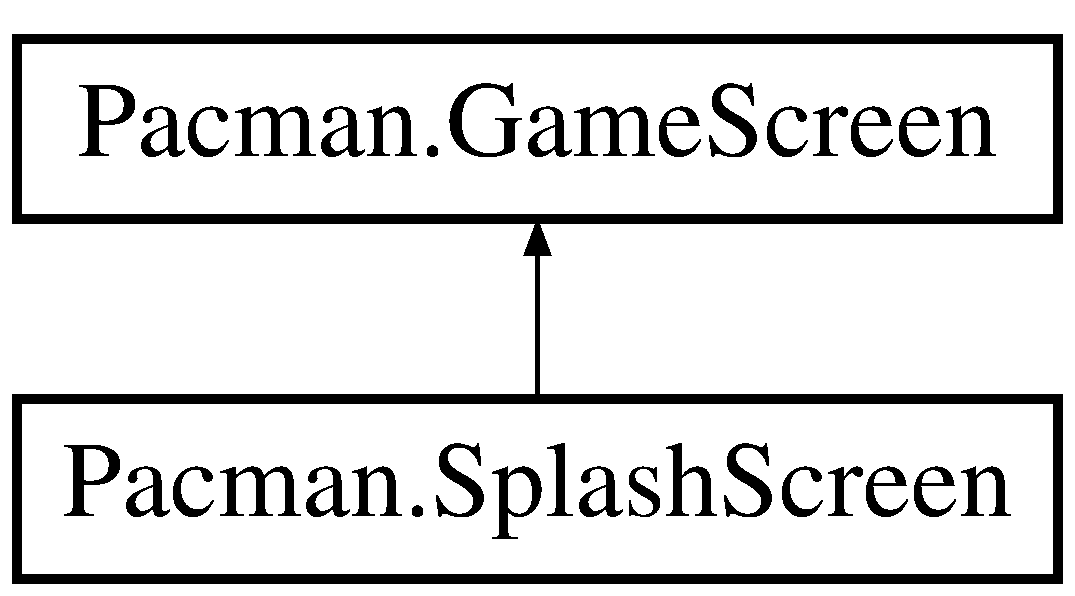
\includegraphics[height=2.000000cm]{class_pacman_1_1_splash_screen}
\end{center}
\end{figure}
\subsection*{Public Member Functions}
\begin{DoxyCompactItemize}
\item 
override void \hyperlink{class_pacman_1_1_splash_screen_a05a5f91c7e0ded6cb4893da9eeb0ded1}{Load\-Content} (Content\-Manager Content)
\begin{DoxyCompactList}\small\item\em Loads the Splash screen images that will be transistioned between which are given from the text file. Loads them into their fade animation. \end{DoxyCompactList}\item 
override void \hyperlink{class_pacman_1_1_splash_screen_ac72328daa3003fa228218c65660c8d6c}{Unload\-Content} ()
\begin{DoxyCompactList}\small\item\em Unloads the content, called when a new screen has been added \end{DoxyCompactList}\item 
override void \hyperlink{class_pacman_1_1_splash_screen_af64e74cca5e74b0104f9fe74a21e52ae}{Update} (Game\-Time game\-Time)
\begin{DoxyCompactList}\small\item\em Fades in and out the images until the last screen has been shown then transtition to the Titelscreen \end{DoxyCompactList}\item 
override void \hyperlink{class_pacman_1_1_splash_screen_a669ad3120d15e6eea2636e44d74cdc31}{Draw} (Sprite\-Batch sprite\-Batch)
\begin{DoxyCompactList}\small\item\em Draw the splash screen images \end{DoxyCompactList}\end{DoxyCompactItemize}
\subsection*{Additional Inherited Members}


\subsection{Detailed Description}
A splash screen that is shown before the title screen 



\subsection{Member Function Documentation}
\hypertarget{class_pacman_1_1_splash_screen_a669ad3120d15e6eea2636e44d74cdc31}{\index{Pacman\-::\-Splash\-Screen@{Pacman\-::\-Splash\-Screen}!Draw@{Draw}}
\index{Draw@{Draw}!Pacman::SplashScreen@{Pacman\-::\-Splash\-Screen}}
\subsubsection[{Draw}]{\setlength{\rightskip}{0pt plus 5cm}override void Pacman.\-Splash\-Screen.\-Draw (
\begin{DoxyParamCaption}
\item[{Sprite\-Batch}]{sprite\-Batch}
\end{DoxyParamCaption}
)\hspace{0.3cm}{\ttfamily [virtual]}}}\label{class_pacman_1_1_splash_screen_a669ad3120d15e6eea2636e44d74cdc31}


Draw the splash screen images 


\begin{DoxyParams}{Parameters}
{\em sprite\-Batch} & \\
\hline
\end{DoxyParams}


Reimplemented from \hyperlink{class_pacman_1_1_game_screen_ab7d62816f246e29e70d352d094c36b04}{Pacman.\-Game\-Screen}.

\hypertarget{class_pacman_1_1_splash_screen_a05a5f91c7e0ded6cb4893da9eeb0ded1}{\index{Pacman\-::\-Splash\-Screen@{Pacman\-::\-Splash\-Screen}!Load\-Content@{Load\-Content}}
\index{Load\-Content@{Load\-Content}!Pacman::SplashScreen@{Pacman\-::\-Splash\-Screen}}
\subsubsection[{Load\-Content}]{\setlength{\rightskip}{0pt plus 5cm}override void Pacman.\-Splash\-Screen.\-Load\-Content (
\begin{DoxyParamCaption}
\item[{Content\-Manager}]{Content}
\end{DoxyParamCaption}
)\hspace{0.3cm}{\ttfamily [virtual]}}}\label{class_pacman_1_1_splash_screen_a05a5f91c7e0ded6cb4893da9eeb0ded1}


Loads the Splash screen images that will be transistioned between which are given from the text file. Loads them into their fade animation. 


\begin{DoxyParams}{Parameters}
{\em Content} & \\
\hline
\end{DoxyParams}


Reimplemented from \hyperlink{class_pacman_1_1_game_screen_a33dbdc943439ae7728aff62b5152aa53}{Pacman.\-Game\-Screen}.

\hypertarget{class_pacman_1_1_splash_screen_ac72328daa3003fa228218c65660c8d6c}{\index{Pacman\-::\-Splash\-Screen@{Pacman\-::\-Splash\-Screen}!Unload\-Content@{Unload\-Content}}
\index{Unload\-Content@{Unload\-Content}!Pacman::SplashScreen@{Pacman\-::\-Splash\-Screen}}
\subsubsection[{Unload\-Content}]{\setlength{\rightskip}{0pt plus 5cm}override void Pacman.\-Splash\-Screen.\-Unload\-Content (
\begin{DoxyParamCaption}
{}
\end{DoxyParamCaption}
)\hspace{0.3cm}{\ttfamily [virtual]}}}\label{class_pacman_1_1_splash_screen_ac72328daa3003fa228218c65660c8d6c}


Unloads the content, called when a new screen has been added 



Reimplemented from \hyperlink{class_pacman_1_1_game_screen_aa33ba4650a38762eca4bd059fb803942}{Pacman.\-Game\-Screen}.

\hypertarget{class_pacman_1_1_splash_screen_af64e74cca5e74b0104f9fe74a21e52ae}{\index{Pacman\-::\-Splash\-Screen@{Pacman\-::\-Splash\-Screen}!Update@{Update}}
\index{Update@{Update}!Pacman::SplashScreen@{Pacman\-::\-Splash\-Screen}}
\subsubsection[{Update}]{\setlength{\rightskip}{0pt plus 5cm}override void Pacman.\-Splash\-Screen.\-Update (
\begin{DoxyParamCaption}
\item[{Game\-Time}]{game\-Time}
\end{DoxyParamCaption}
)\hspace{0.3cm}{\ttfamily [virtual]}}}\label{class_pacman_1_1_splash_screen_af64e74cca5e74b0104f9fe74a21e52ae}


Fades in and out the images until the last screen has been shown then transtition to the Titelscreen 


\begin{DoxyParams}{Parameters}
{\em game\-Time} & \\
\hline
\end{DoxyParams}


Reimplemented from \hyperlink{class_pacman_1_1_game_screen_a768b26cbc3ed823d0dcba5055ae9a8b4}{Pacman.\-Game\-Screen}.



The documentation for this class was generated from the following file\-:\begin{DoxyCompactItemize}
\item 
Splash\-Screen.\-cs\end{DoxyCompactItemize}

\hypertarget{class_pacman_1_1_titel_screen}{\section{Pacman.\-Titel\-Screen Class Reference}
\label{class_pacman_1_1_titel_screen}\index{Pacman.\-Titel\-Screen@{Pacman.\-Titel\-Screen}}
}


Titel screen, shown after the splash screen before the main menu screen  


Inheritance diagram for Pacman.\-Titel\-Screen\-:\begin{figure}[H]
\begin{center}
\leavevmode
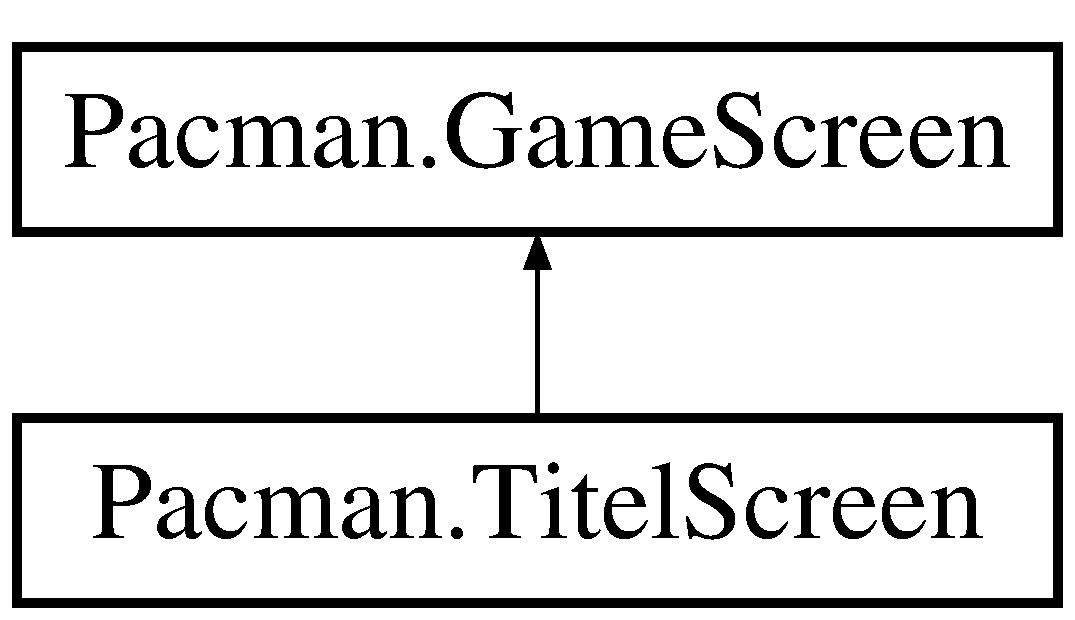
\includegraphics[height=2.000000cm]{class_pacman_1_1_titel_screen}
\end{center}
\end{figure}
\subsection*{Public Member Functions}
\begin{DoxyCompactItemize}
\item 
override void \hyperlink{class_pacman_1_1_titel_screen_aaeeb7b4a31657e20e6d37926d38e5c31}{Load\-Content} (Content\-Manager Content)
\begin{DoxyCompactList}\small\item\em Loads the text fade and screen fade animation. Loads in a computer contoled character animation. \end{DoxyCompactList}\item 
override void \hyperlink{class_pacman_1_1_titel_screen_ae9feed8a91c5fe3da560994fe4258fb2}{Unload\-Content} ()
\begin{DoxyCompactList}\small\item\em Unloads the content and fade animations. \end{DoxyCompactList}\item 
override void \hyperlink{class_pacman_1_1_titel_screen_a287b7f099f4336dbc7b4e232d062441a}{Update} (Game\-Time game\-Time)
\begin{DoxyCompactList}\small\item\em Updates the fade animations and the character animation and it's position. And checks if the user has pressed the Enter key transitions to the main menu screen. \end{DoxyCompactList}\item 
override void \hyperlink{class_pacman_1_1_titel_screen_ae86c21742cdd405fd4467b67b509bc6d}{Draw} (Sprite\-Batch sprite\-Batch)
\begin{DoxyCompactList}\small\item\em Draws the fade animations and the character animations. \end{DoxyCompactList}\end{DoxyCompactItemize}
\subsection*{Additional Inherited Members}


\subsection{Detailed Description}
Titel screen, shown after the splash screen before the main menu screen 



\subsection{Member Function Documentation}
\hypertarget{class_pacman_1_1_titel_screen_ae86c21742cdd405fd4467b67b509bc6d}{\index{Pacman\-::\-Titel\-Screen@{Pacman\-::\-Titel\-Screen}!Draw@{Draw}}
\index{Draw@{Draw}!Pacman::TitelScreen@{Pacman\-::\-Titel\-Screen}}
\subsubsection[{Draw}]{\setlength{\rightskip}{0pt plus 5cm}override void Pacman.\-Titel\-Screen.\-Draw (
\begin{DoxyParamCaption}
\item[{Sprite\-Batch}]{sprite\-Batch}
\end{DoxyParamCaption}
)\hspace{0.3cm}{\ttfamily [virtual]}}}\label{class_pacman_1_1_titel_screen_ae86c21742cdd405fd4467b67b509bc6d}


Draws the fade animations and the character animations. 


\begin{DoxyParams}{Parameters}
{\em sprite\-Batch} & \\
\hline
\end{DoxyParams}


Reimplemented from \hyperlink{class_pacman_1_1_game_screen_ab7d62816f246e29e70d352d094c36b04}{Pacman.\-Game\-Screen}.

\hypertarget{class_pacman_1_1_titel_screen_aaeeb7b4a31657e20e6d37926d38e5c31}{\index{Pacman\-::\-Titel\-Screen@{Pacman\-::\-Titel\-Screen}!Load\-Content@{Load\-Content}}
\index{Load\-Content@{Load\-Content}!Pacman::TitelScreen@{Pacman\-::\-Titel\-Screen}}
\subsubsection[{Load\-Content}]{\setlength{\rightskip}{0pt plus 5cm}override void Pacman.\-Titel\-Screen.\-Load\-Content (
\begin{DoxyParamCaption}
\item[{Content\-Manager}]{Content}
\end{DoxyParamCaption}
)\hspace{0.3cm}{\ttfamily [virtual]}}}\label{class_pacman_1_1_titel_screen_aaeeb7b4a31657e20e6d37926d38e5c31}


Loads the text fade and screen fade animation. Loads in a computer contoled character animation. 


\begin{DoxyParams}{Parameters}
{\em Content} & \\
\hline
\end{DoxyParams}


Reimplemented from \hyperlink{class_pacman_1_1_game_screen_a33dbdc943439ae7728aff62b5152aa53}{Pacman.\-Game\-Screen}.

\hypertarget{class_pacman_1_1_titel_screen_ae9feed8a91c5fe3da560994fe4258fb2}{\index{Pacman\-::\-Titel\-Screen@{Pacman\-::\-Titel\-Screen}!Unload\-Content@{Unload\-Content}}
\index{Unload\-Content@{Unload\-Content}!Pacman::TitelScreen@{Pacman\-::\-Titel\-Screen}}
\subsubsection[{Unload\-Content}]{\setlength{\rightskip}{0pt plus 5cm}override void Pacman.\-Titel\-Screen.\-Unload\-Content (
\begin{DoxyParamCaption}
{}
\end{DoxyParamCaption}
)\hspace{0.3cm}{\ttfamily [virtual]}}}\label{class_pacman_1_1_titel_screen_ae9feed8a91c5fe3da560994fe4258fb2}


Unloads the content and fade animations. 



Reimplemented from \hyperlink{class_pacman_1_1_game_screen_aa33ba4650a38762eca4bd059fb803942}{Pacman.\-Game\-Screen}.

\hypertarget{class_pacman_1_1_titel_screen_a287b7f099f4336dbc7b4e232d062441a}{\index{Pacman\-::\-Titel\-Screen@{Pacman\-::\-Titel\-Screen}!Update@{Update}}
\index{Update@{Update}!Pacman::TitelScreen@{Pacman\-::\-Titel\-Screen}}
\subsubsection[{Update}]{\setlength{\rightskip}{0pt plus 5cm}override void Pacman.\-Titel\-Screen.\-Update (
\begin{DoxyParamCaption}
\item[{Game\-Time}]{game\-Time}
\end{DoxyParamCaption}
)\hspace{0.3cm}{\ttfamily [virtual]}}}\label{class_pacman_1_1_titel_screen_a287b7f099f4336dbc7b4e232d062441a}


Updates the fade animations and the character animation and it's position. And checks if the user has pressed the Enter key transitions to the main menu screen. 


\begin{DoxyParams}{Parameters}
{\em game\-Time} & \\
\hline
\end{DoxyParams}


Reimplemented from \hyperlink{class_pacman_1_1_game_screen_a768b26cbc3ed823d0dcba5055ae9a8b4}{Pacman.\-Game\-Screen}.



The documentation for this class was generated from the following file\-:\begin{DoxyCompactItemize}
\item 
Titel\-Screen.\-cs\end{DoxyCompactItemize}

%--- End generated contents ---

% Index
\newpage
\phantomsection
\addcontentsline{toc}{part}{Index}
\printindex

\end{document}
